%% LyX 2.4.3 created this file.  For more info, see https://www.lyx.org/.
%% Do not edit unless you really know what you are doing.
\documentclass[journal,article,submit,pdftex,moreauthors]{Definitions/mdpi}
\usepackage[utf8]{inputenc}
\usepackage{float}
\usepackage{url}
\usepackage{amsmath}
\usepackage{graphicx}

\makeatletter

%%%%%%%%%%%%%%%%%%%%%%%%%%%%%% LyX specific LaTeX commands.

\Title{From Initialization to Convergence: A Three-Stage technique for Robust
RBF Network Training}

\TitleCitation{From Initialization to Convergence: A Three-Stage technique for Robust
RBF Network Training}

\Author{Ioannis G. Tsoulos$^{1,*}$, Vasileios Charilogis$^{2}$, Dimitrios
Tsalikakis$^{3}$}

\AuthorNames{Ioannis G. Tsoulos, Vasileios Charilogis, Dimitrios Tsalikakis}

\AuthorCitation{Tsoulos, I.G.; Charilogis, V.; Tsalikakis D.}


\address{$^{1}$\quad{}Department of Informatics and Telecommunications,
University of Ioannina, Greece;itsoulos@uoi.gr\\
$^{2}$\quad{}Department of Informatics and Telecommunications, University
of Ioannina, Greece; v.charilog@uoi.gr\\
$^{3}\quad$Department of Engineering Informatics and Telecommunications,
University of Western Macedonia, 50100 Kozani, Greece; dtsalikakis@uowm.gr}


\corres{Correspondence: itsoulos@uoi.gr}


\abstract{Radial Basis Function (RBF) networks are well established machine
learning tools used in a variety of classification and regression
problems. A key component of these networks is their radial functions.
These networks acquire adaptive capabilities through a two-stage training
technique in most cases. In the first stage, the centers and variances
for the radial functions are estimated, and in the second stage, through
the solution of a linear system, the external weights for the radial
functions are adjusted. However, in many cases this training technique
has reduced performance either due to instability in arithmetic operations
or due to trapping in local minima of the training error. In this
paper, a three-stage method is proposed to address the above problems.
In the first stage, an initial estimate of the intervals for the network
parameter values \LyXZeroWidthSpace\LyXZeroWidthSpace is made, in
the second stage, the network parameter values are adjusted within
the intervals of the first phase, and finally in the third stage of
the proposed technique, a local optimization method is used for the
final adjustment of the network parameters. The proposed method was
tested for its efficiency on a wide series of regression and classification
datasets from the related bibliography with exceptional results. }


\keyword{Machine learning; Neural networks; Genetic algorithms; Optimization}

\newcommand*\LyXZeroWidthSpace{\hspace{0pt}}
\DeclareTextSymbolDefault{\textquotedbl}{T1}
%% Because html converters don't know tabularnewline
\providecommand{\tabularnewline}{\\}
\floatstyle{ruled}
\newfloat{algorithm}{tbp}{loa}
\providecommand{\algorithmname}{Algorithm}
\floatname{algorithm}{\protect\algorithmname}

%%%%%%%%%%%%%%%%%%%%%%%%%%%%%% User specified LaTeX commands.
%  LaTeX support: latex@mdpi.com 
%  For support, please attach all files needed for compiling as well as the log file, and specify your operating system, LaTeX version, and LaTeX editor.

%=================================================================
%\documentclass[preprints,article,submit,pdftex,moreauthors]{Definitions/mdpi} 
% For posting an early version of this manuscript as a preprint, you may use "preprints" as the journal. Changing "submit" to "accept" before posting will remove line numbers.

% Below journals will use APA reference format:
% admsci, aichem, behavsci, businesses, econometrics, economies, education, ejihpe, famsci, games, humans, ijcs, ijfs, journalmedia, jrfm, languages, psycholint, publications, tourismhosp, youth

% Below journals will use Chicago reference format:
% arts, genealogy, histories, humanities, jintelligence, laws, literature, religions, risks, socsci

%--------------------
% Class Options:
%--------------------
%----------
% journal
%----------
% Choose between the following MDPI journals:
% accountaudit, acoustics, actuators, addictions, adhesives, admsci, adolescents, aerobiology, aerospace, agriculture, agriengineering, agrochemicals, agronomy, ai, air, algorithms, allergies, alloys, amh, analytica, analytics, anatomia, anesthres, animals, antibiotics, antibodies, antioxidants, applbiosci, appliedchem, appliedmath, appliedphys, applmech, applmicrobiol, applnano, applsci, aquacj, architecture, arm, arthropoda, arts, asc, asi, astronomy, atmosphere, atoms, audiolres, automation, axioms, bacteria, batteries, bdcc, behavsci, beverages, biochem, bioengineering, biologics, biology, biomass, biomechanics, biomed, biomedicines, biomedinformatics, biomimetics, biomolecules, biophysica, biosensors, biosphere, biotech, birds, blockchains, bloods, blsf, brainsci, breath, buildings, businesses, cancers, carbon, cardiogenetics, catalysts, cells, ceramics, challenges, chemengineering, chemistry, chemosensors, chemproc, children, chips, cimb, civileng, cleantechnol, climate, clinbioenerg, clinpract, clockssleep, cmd, cmtr, coasts, coatings, colloids, colorants, commodities, complications, compounds, computation, computers, condensedmatter, conservation, constrmater, cosmetics, covid, crops, cryo, cryptography, crystals, csmf, ctn, curroncol, cyber, dairy, data, ddc, dentistry, dermato, dermatopathology, designs, devices, diabetology, diagnostics, dietetics, digital, disabilities, diseases, diversity, dna, drones, dynamics, earth, ebj, ecm, ecologies, econometrics, economies, education, eesp, ejihpe, electricity, electrochem, electronicmat, electronics, encyclopedia, endocrines, energies, eng, engproc, ent, entomology, entropy, environments, epidemiologia, epigenomes, esa, est, famsci, fermentation, fibers, fintech, fire, fishes, fluids, foods, forecasting, forensicsci, forests, fossstud, foundations, fractalfract, fuels, future, futureinternet, futureparasites, futurepharmacol, futurephys, futuretransp, galaxies, games, gases, gastroent, gastrointestdisord, gastronomy, gels, genealogy, genes, geographies, geohazards, geomatics, geometry, geosciences, geotechnics, geriatrics, glacies, grasses, greenhealth, gucdd, hardware, hazardousmatters, healthcare, hearts, hemato, hematolrep, heritage, higheredu, highthroughput, histories, horticulturae, hospitals, humanities, humans, hydrobiology, hydrogen, hydrology, hygiene, idr, iic, ijerph, ijfs, ijgi, ijmd, ijms, ijns, ijpb, ijt, ijtm, ijtpp, ime, immuno, informatics, information, infrastructures, inorganics, insects, instruments, inventions, iot, j, jal, jcdd, jcm, jcp, jcs, jcto, jdad, jdb, jeta, jfb, jfmk, jimaging, jintelligence, jlpea, jmahp, jmmp, jmms, jmp, jmse, jne, jnt, jof, joitmc, joma, jop, jor, journalmedia, jox, jpbi, jpm, jrfm, jsan, jtaer, jvd, jzbg, kidney, kidneydial, kinasesphosphatases, knowledge, labmed, laboratories, land, languages, laws, life, lights, limnolrev, lipidology, liquids, literature, livers, logics, logistics, lubricants, lymphatics, machines, macromol, magnetism, magnetochemistry, make, marinedrugs, materials, materproc, mathematics, mca, measurements, medicina, medicines, medsci, membranes, merits, metabolites, metals, meteorology, methane, metrics, metrology, micro, microarrays, microbiolres, microelectronics, micromachines, microorganisms, microplastics, microwave, minerals, mining, mmphys, modelling, molbank, molecules, mps, msf, mti, multimedia, muscles, nanoenergyadv, nanomanufacturing, nanomaterials, ncrna, ndt, network, neuroglia, neurolint, neurosci, nitrogen, notspecified, nursrep, nutraceuticals, nutrients, obesities, oceans, ohbm, onco, oncopathology, optics, oral, organics, organoids, osteology, oxygen, parasites, parasitologia, particles, pathogens, pathophysiology, pediatrrep, pets, pharmaceuticals, pharmaceutics, pharmacoepidemiology, pharmacy, philosophies, photochem, photonics, phycology, physchem, physics, physiologia, plants, plasma, platforms, pollutants, polymers, polysaccharides, populations, poultry, powders, preprints, proceedings, processes, prosthesis, proteomes, psf, psych, psychiatryint, psychoactives, psycholint, publications, purification, quantumrep, quaternary, qubs, radiation, reactions, realestate, receptors, recycling, regeneration, religions, remotesensing, reports, reprodmed, resources, rheumato, risks, robotics, rsee, ruminants, safety, sci, scipharm, sclerosis, seeds, sensors, separations, sexes, signals, sinusitis, siuj, skins, smartcities, sna, societies, socsci, software, soilsystems, solar, solids, spectroscj, sports, standards, stats, std, stresses, surfaces, surgeries, suschem, sustainability, symmetry, synbio, systems, tae, targets, taxonomy, technologies, telecom, test, textiles, thalassrep, therapeutics, thermo, timespace, tomography, tourismhosp, toxics, toxins, transplantology, transportation, traumacare, traumas, tropicalmed, universe, urbansci, uro, vaccines, vehicles, venereology, vetsci, vibration, virtualworlds, viruses, vision, waste, water, wem, wevj, wild, wind, women, world, youth, zoonoticdis

%---------
% article
%---------
% The default type of manuscript is "article", but can be replaced by: 
% abstract, addendum, article, book, bookreview, briefreport, casereport, comment, commentary, communication, conferenceproceedings, correction, conferencereport, entry, expressionofconcern, extendedabstract, datadescriptor, editorial, essay, erratum, hypothesis, interestingimage, obituary, opinion, projectreport, reply, retraction, review, perspective, protocol, shortnote, studyprotocol, systematicreview, supfile, technicalnote, viewpoint, guidelines, registeredreport, tutorial
% supfile = supplementary materials

%----------
% submit
%----------
% The class option "submit" will be changed to "accept" by the Editorial Office when the paper is accepted. This will only make changes to the frontpage (e.g., the logo of the journal will get visible), the headings, and the copyright information. Also, line numbering will be removed. Journal info and pagination for accepted papers will also be assigned by the Editorial Office.

%------------------
% moreauthors
%------------------
% If there is only one author the class option oneauthor should be used. Otherwise use the class option moreauthors.

%---------
% pdftex
%---------
% The option pdftex is for use with pdfLaTeX. If eps figures are used, remove the option pdftex and use LaTeX and dvi2pdf.

%=================================================================
% MDPI internal commands - do not modify
\firstpage{1} 
\setcounter{page}{\@firstpage}
\pubvolume{1}
\issuenum{1}
\articlenumber{0}
\pubyear{2025}
\copyrightyear{2025}
%\externaleditor{Firstname Lastname} % More than 1 editor, please add `` and '' before the last editor name
\datereceived{}
\daterevised{ } % Comment out if no revised date
\dateaccepted{}
\datepublished{}
%\datecorrected{} % For corrected papers include a "Corrected: XXX" date in the original paper.
%\dateretracted{} % For retracted papers include a "RETRACTED: XXX" date in the original paper.
\hreflink{https://doi.org/} % If needed use \linebreak
%\doinum{}
%\pdfoutput=1 % Uncommented for upload to arXiv.org
%\CorrStatement{yes}  % For updates
%\longauthorlist{yes} % For many authors that exceed the left citation part

%=================================================================
% Add packages and commands here. The following packages are loaded in our class file: fontenc, inputenc, calc, indentfirst, fancyhdr, graphicx, epstopdf, lastpage, ifthen, lineno, float, amsmath, setspace, enumitem, mathpazo, booktabs, titlesec, etoolbox, tabto, xcolor, soul, multirow, microtype, tikz, totcount, changepage, attrib, upgreek, cleveref, amsthm, hyphenat, natbib, hyperref, footmisc, url, geometry, newfloat, caption

%=================================================================
%% Please use the following mathematics environments: Theorem, Lemma, Corollary, Proposition, Characterization, Property, Problem, Example, ExamplesandDefinitions, Hypothesis, Remark, Definition, Notation, Assumption
%% For proofs, please use the proof environment (the amsthm package is loaded by the MDPI class).

%=================================================================
% The fields PACS, MSC, and JEL may be left empty or commented out if not applicable
%\PACS{J0101}
%\MSC{}
%\JEL{}

%%%%%%%%%%%%%%%%%%%%%%%%%%%%%%%%%%%%%%%%%%
% Only for the journal Diversity
%\LSID{\url{http://}}

%%%%%%%%%%%%%%%%%%%%%%%%%%%%%%%%%%%%%%%%%%
% Only for the journal Applied Sciences:
%\featuredapplication{Authors are encouraged to provide a concise description of the specific application or a potential application of the work. This section is not mandatory.}
%%%%%%%%%%%%%%%%%%%%%%%%%%%%%%%%%%%%%%%%%%

%%%%%%%%%%%%%%%%%%%%%%%%%%%%%%%%%%%%%%%%%%
% Only for the journal Data:
%\dataset{DOI number or link to the deposited data set in cases where the data set is published or set to be published separately. If the data set is submitted and will be published as a supplement to this paper in the journal Data, this field will be filled by the editors of the journal. In this case, please make sure to submit the data set as a supplement when entering your manuscript into our manuscript editorial system.}

%\datasetlicense{license under which the data set is made available (CC0, CC-BY, CC-BY-SA, CC-BY-NC, etc.)}

%%%%%%%%%%%%%%%%%%%%%%%%%%%%%%%%%%%%%%%%%%
% Only for the journal BioTech, Fishes, Neuroimaging and Toxins
%\keycontribution{The breakthroughs or highlights of the manuscript. Authors can write one or two sentences to describe the most important part of the paper.}

%%%%%%%%%%%%%%%%%%%%%%%%%%%%%%%%%%%%%%%%%%
% Only for the journal Encyclopedia
%\encyclopediadef{Instead of the abstract}
%\entrylink{The Link to this entry published on the encyclopedia platform.}
%%%%%%%%%%%%%%%%%%%%%%%%%%%%%%%%%%%%%%%%%%

%%%%%%%%%%%%%%%%%%%%%%%%%%%%%%%%%%%%%%%%%%
% Only for the journal Advances in Respiratory Medicine, Future, Sensors and Smart Cities
%\addhighlights{yes}
%\renewcommand{\addhighlights}{%

%\noindent This is an obligatory section in ``Advances in Respiratory Medicine'', ``Future'', ``Sensors'' and ``Smart Cities”, whose goal is to increase the discoverability and readability of the article via search engines and other scholars. Highlights should not be a copy of the abstract, but a simple text allowing the reader to quickly and simplified find out what the article is about and what can be cited from it. Each of these parts should be devoted up to 2~bullet points.\vspace{3pt}\\
%\textbf{What are the main findings?}
% \begin{itemize}[labelsep=2.5mm,topsep=-3pt]
% \item First bullet.
% \item Second bullet.
% \end{itemize}\vspace{3pt}
%\textbf{What is the implication of the main finding?}
% \begin{itemize}[labelsep=2.5mm,topsep=-3pt]
% \item First bullet.
% \item Second bullet.
% \end{itemize}
%}
%%%%%%%%%%%%%%%%%%%%%%%%%%%%%%%%%%%%%%%%%%

\makeatother

\begin{document}
\maketitle

\section{Introduction}

Many practical problems can be tackled by machine learning models,
such as problems occurred in physics \citep{physics_ml1,physics_ml2},
astronomy \citep{astronomy_ml1,astronomy_ml2}, chemistry \citep{chemistry_ml1,chemistry_ml2},
medicine \citep{med_ml1,med_ml2}, economics \citep{econ_ml1,econ_ml2},
image processing \citep{nn_image}, time series forecasting \citep{nn_timeseries}
etc. Among the most used machine learning tools one can detect the
Radial Basis Function (RBF) networks, expressed using the following
definition:
\begin{equation}
R\left(\overrightarrow{x}\right)=\sum_{i=1}^{k}w_{i}\phi\left(\left\Vert \overrightarrow{x}-\overrightarrow{c_{i}}\right\Vert \right)\label{eq:firstrbf}
\end{equation}
The symbols appeared in this equation are defined as follows:
\begin{enumerate}
\item The vector $\overrightarrow{x}$ stands for the input pattern. The
dimension of each pattern is denoted by $d$.
\item The constant $k$ denotes number of weights of the network. The vector
$\overrightarrow{w}$ denotes these weights.
\item The vectors $\overrightarrow{c_{i}},\ i=1,..,k$ denote the centers
of the network.
\item The function $\phi(x)$ usually represents a Gaussian function having
the following form:\textbf{ }
\begin{equation}
\phi(x)=\exp\left(-\frac{\left(x-c\right)^{2}}{\sigma^{2}}\right)
\end{equation}
\end{enumerate}
A plot of the Gaussian function $c=0,\ \sigma=1$ is shown in Figure
\ref{fig:gaussian}. 
\begin{figure}[H]
\begin{centering}
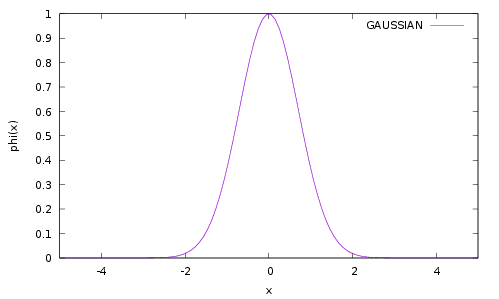
\includegraphics{gaussian}
\par\end{centering}
\caption{A typical plot for the Gaussian function.\label{fig:gaussian}}
\end{figure}
 This graph clearly shows that the value of the function decreases
as the value of x moves away from the center $c$. The training error
of any given $R(x)$ RBF network is defined as:
\begin{equation}
E\left(R\left(\overrightarrow{x}\right)\right)=\sum_{i=1}^{M}\left(R\left(\overrightarrow{x_{i}}\right)-y_{i}\right)^{2}\label{eq:RbfError}
\end{equation}
The set $\left(\overrightarrow{x_{i}},y_{i}\right),\ i=1,...,M$ denotes
the training set of the objective problem and the values $y_{i}$
are considered as the actual output for each pattern $\overrightarrow{x_{i}}$.

RBF networks have been used in many cases, such as face recognition
\citep{rbfface}, solutions of differential equations \citep{rbfde1,rbfde2},
stock prediction \citep{rbfstock}, robotics \citep{rbfrobotics1,rbfrobotics2},
network security \citep{rbf_dos1,rbf_dos2}, classification of process
faults \citep{rbf_process}, time series prediction \citep{rbf_time},
estimation of wind power production \citep{rbf_wind} etc. Moreover,
Park et al \citep{rbf_universal} proved that an RBF network with
one processing layer is capable of universal approximation.

Recently, a series of papers have been proposed for the initialization
of the parameters of RBF networks \citep{rbfinit1,rbfinit2,rbfinit3}.
Moreover,\textbf{ }Benoudjit et al provided a discussion on the estimation
of kernel widths in RBF networks \citep{rbfkernel}. Additionally,
a series of pruning techniques\textbf{ }\citep{rbfprun1,rbfprun2,rbfprun3}
have been introduced aiming to reduce the number of parameters of
the RBF networks in order to avoid the overfitting problem. Also,
a series of optimization techniques have been incorporated in the
past to tackle the equation \ref{eq:RbfError}, such as Genetic algorithms
\citep{rbfga1,rbfga2}, the Particle Swam Optimization method \citep{rbfpso1,rbfpso2},
the Differential Evolution technique \citep{rbfdiff1} etc. Furthermore,
the rapid increase in the use of parallel computing techniques in
recent decades has resulted in the publication of a series of relevant
scientific papers that exploit this techniques\textbf{ }\citep{rbfpar1,rbfpar2}.

In this paper, the use of a three-stage technique is proposed for
the effective training of RBF networks. In the first stage of the
technique, the range of values for the parameters of the RBF network
is detected. This detection is implemented using the K-Means algorithm
\citep{kmeans} for the weights and the variances of the radial functions.
After applying the above procedure, a range of values for the network
parameters is created which directly depends on the values produced
by K-means algorithm. During the second stage of the proposed work,
a global optimization procedure is incorporated to optimize the parameters
of the RBF network with respect to equation \ref{eq:RbfError}. The
training of the parameters is performed inside the interval of values
created during the first stage of the technique. In the current work
the Genetic Algorithm is used as the method of the second phase, but
any optimization technique can be incorporated. Finally, in the third
stage of the proposed work, a local optimization procedure is applied
to the best solution located in the second phase. The purpose of the
present technique is first to identify a reliable range of values
\LyXZeroWidthSpace\LyXZeroWidthSpace for the parameters of RBF networks
and then to train the network parameters within this range of values,
avoiding possible arithmetic instability problems presented by the
established method of training RBF networks.

The remaining of this article is organized as follows: in section
\ref{sec:Materials-and-Methods} the proposed method and the accompanied
genetic algorithm are introduced, in section \ref{sec:Results} the
experimental datasets and the series of experiments conducted are
listed and discussed thoroughly followed by section \ref{sec:Conclusions}
where some conclusions are discussed.

\section{Materials and Methods\label{sec:Materials-and-Methods}}

The three distinct phases of the proposed method are analyzed in this
section. The discussion initiates with the first phase, where the
construction of the ranges for the parameter values is performed using
the K-means algorithm. Subsequently, the steps of the used Genetic
Algorithm are presented in detail and finally this section concludes
with the description of the final phase, where a local optimization
method is applied to the best located chromosome of the second phase.

\subsection{The first phase of the proposed method }

The method of K-means, used widely in machine learning is incorporated
in the first phase for the location of the ranges for the parameters
of the RBF network. This method is incorporated to locate the centers
and the variances of the possible groups of a series of points. Furthermore,
a series of extensions of this method have been published during the
past years, such as the Genetic K-means algotithm \citep{gen_kmeans},
the unsupervised K-means algorithm \citep{unsuper_kmeans}, the Fixed-centered
K-means algorithm \citep{fixed_kmeans} etc. A detailed review for
the K-means method can be be located in the work of Oti et al. \citep{kmeans_review}.
The K-means method is presented in Algorithm \ref{alg:The-K-Means-algorithm.}
and a graphical rerpesentation is provided in Figure \ref{fig:kmeans}.

\begin{algorithm}[H]
\caption{The main steps of the K-means algorithm.\label{alg:The-K-Means-algorithm.}}

\begin{enumerate}
\item \textbf{Input: }The set of patterns of the objective problem\textbf{
$\left(\overrightarrow{x_{i}}\right),\ i=1,...,M$}
\item \textbf{Input}: the number of centers $k$.
\item \textbf{Output}: The vectors $\overrightarrow{c_{i}},\ i=1,..,k$
and the quantities $\sigma_{i},\ i=1,\ldots,k$
\item \textbf{Set} $S_{j}=\left\{ \right\} ,\ j=1..k$, as the sets of samples
belonging to the same group.
\item \textbf{For} each pattern $x_{i},\ i=1,...,M$ \textbf{do\label{enu:For-every-pattern}}
\begin{enumerate}
\item \textbf{Set} $j^{*}=\min_{i=1}^{k}\left\{ D\left(x_{i},c_{j}\right)\right\} $.
\item \textbf{Set} $S_{j^{*}}=S_{j^{*}}\cup\left\{ x_{i}\right\} $.
\end{enumerate}
\item \textbf{EndFor}
\item \textbf{For} each center $c_{j},\ j=1..k$ \textbf{do}
\begin{enumerate}
\item \textbf{Calculate} as $M_{j}$ the number of points belonging to the
group $S_{j}$
\item \textbf{Compute }$c_{j}$ as
\[
c_{j}=\frac{1}{M_{j}}\sum_{i=1}^{M_{j}}x_{i}
\]
\end{enumerate}
\item \textbf{EndFor}
\item \textbf{Calculate} the quantities $s_{j}$ as 
\[
\sigma_{j}^{2}=\frac{\sum_{i=1}^{M_{j}}\left(x_{i}-c_{j}\right)^{2}}{M_{j}}
\]
\item \textbf{Stop }the algorithm, if there is no change in centers $c_{j}$.
\item \textbf{Go to} step \ref{enu:For-every-pattern}.
\end{enumerate}
\end{algorithm}
\begin{figure}[H]
\begin{centering}
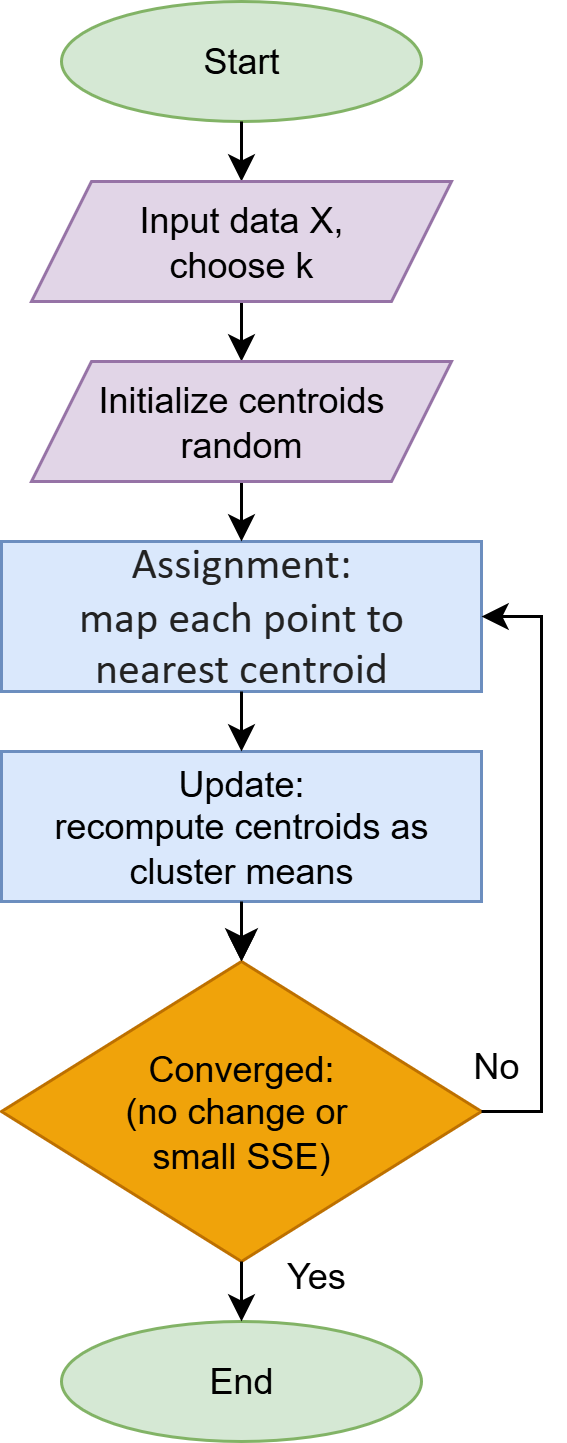
\includegraphics[scale=0.75]{kmeans_flowchart}
\par\end{centering}
\caption{A graphical presentation of the K-means algorithm. \label{fig:kmeans}}
\end{figure}

After the calculation of $\overrightarrow{c_{i}},\ i=1,..,k$ and
the quantities $\sigma_{i},\ i=1,\ldots,k$, the method locates the
bound vectors $\overrightarrow{L},\ \overrightarrow{R}$ for the parameters
of the RBF network. The dimension of the bound vectors is defined
as:
\begin{equation}
n=(d+2)\times k\label{eq:bound_dimension}
\end{equation}
For the calculation of the bound vectors the procedure presented in
Algorithm \ref{alg:initialValues} is utilized.

\begin{algorithm}[H]
\caption{Algorithm used to obtain the bound vectors $\protect\overrightarrow{L},\ \protect\overrightarrow{R}$
\label{alg:initialValues}}

\begin{enumerate}
\item \textbf{Input:} The vectors $\overrightarrow{c_{i}},\ i=1,..,k$ and
the quantities $\sigma_{i},\ i=1,\ldots,k$ of the K-means procedure.
\item \textbf{Input}: the initial bound for the weight vector $\overrightarrow{w}$,
denoted as $B_{w}>0$.
\item \textbf{Input}: the scaling factor $F\ge1$.
\item \textbf{Output:} the vectors $\overrightarrow{L},\ \overrightarrow{R}$.
\item \textbf{Set} $m=0$
\item \textbf{For} $i=1..k$ \textbf{do}
\begin{enumerate}
\item \textbf{For} $j=1..d$ \textbf{do}
\begin{enumerate}
\item \textbf{Set} $L_{m}$=$-F\times c_{ij}$, $R_{m}$=$F\times c_{ij}$
\item \textbf{Set} $m=m+1$
\end{enumerate}
\item \textbf{EndFor}
\item \textbf{Set} $L_{m}=-F\times\sigma_{i}$, $R_{m}=F\times\sigma_{i}$
\item \textbf{Set} $m=m+1$
\end{enumerate}
\item \textbf{EndFor}
\item \textbf{For} $j=1,...,k$ \textbf{do}
\begin{enumerate}
\item \textbf{Set} $L_{m}=-B_{w},\ R_{m}=B_{w}$
\item \textbf{Set} $m=m+1$
\end{enumerate}
\item \textbf{EndFor}
\end{enumerate}
\end{algorithm}


\subsection{The second phase of the proposed method }

During the second phase an optimization procedure is utilized to minimize
the equation \ref{eq:RbfError} inside the bound vectors $\overrightarrow{L},\ \overrightarrow{R}$
of the first phase. In the proposed implementation the Genetic Algorithm
was incorporated during the second phase. Genetic algorithm are evolutionary
methods, that are based on randomly produced solutions of the objective
problem. These solutions are called chromosomes and they are evolved
through some operations similar to natural processes of selection,
crossover and mutation. Genetic algorithms have been used in a wide
series of problems, such as placement of wind turbines \citep{gen_app1},
water distribution \citep{gen_app2}, problems appeared in banking
transactions \citep{gen_app3}, optimization of neural networks \citep{gen_app4}
etc. Also, another advantage of Genetic Algorithms is that they can
be easily adopt parallel programming techniques in order to speed
up the evolutionary process \citep{pga1,pga2}. The layout of the
chromosomes used in the obtained genetic algorithm is presented in
Figure \ref{fig:The-layout-of}. \textbf{I}n this layout the following
assumptions are hold:
\begin{enumerate}
\item The value $c_{i,j}$ denotes the $j$ element of the $i$ center of
the RBF network, with $i\in[1,k]$ and $j\in[1,d].$
\item The value $\sigma_{i}$ represents the $\sigma$ parameter for the
corresponding radial function.
\item The value $w_{i},\ i\in[1,k]$ represents the weight for the corresponding
radial function.
\end{enumerate}
\begin{figure}[H]

\includegraphics[scale=0.65]{chrom}

\caption{The layout of chromosomes used in the second stage of the proposed
method.\label{fig:The-layout-of}}
\end{figure}

The steps of the genetic algorithm used in the second phase of the
proposed method have as follows:
\begin{enumerate}
\item \textbf{Initialization step}. 
\begin{enumerate}
\item \textbf{Set} the of chromosomes $N_{c}$ and the maximum number of
generations denoted as as $N_{g}$.
\item \textbf{Set} $p_{s}$ the selection rate and as $p_{m}$ the mutation
rate.
\item \textbf{Initialize} every chromosome $g_{i},\ i=1,\ldots,N_{c}$ of
the population as vector of double numbers. The layout of each chromosome
follows the scheme of Figure \ref{fig:The-layout-of} and the initialization
is performed inside the bound vectors $\overrightarrow{L},\ \overrightarrow{R}$.
\item \textbf{Set} $k=0$, the generation number.
\end{enumerate}
\item \textbf{Fitness calculation step}.
\begin{enumerate}
\item \textbf{For} $i=1,\ldots,N_{c}$ \textbf{do}
\begin{enumerate}
\item \textbf{Produce }an RBF network $R_{i}=R\left(\overrightarrow{x},\overrightarrow{g_{i}}\right)$
for the corresponding chromosome $\overrightarrow{g_{i}}.$
\item \textbf{Estimate} the related fitness value $f_{i}$ as\textbf{
\begin{equation}
f_{i}=\sum_{j=1}^{M}\left(R\left(\overrightarrow{x}_{j},\overrightarrow{g_{i}}\right)-y_{j}\right)^{2}\label{eq:eq1-1}
\end{equation}
}
\end{enumerate}
\item \textbf{End For}
\end{enumerate}
\item \textbf{Genetic operations step}.
\begin{enumerate}
\item Selection procedure: During this procedure the chromosomes are sorted
according to their fitness values and the best $p_{s}\times N_{c}$
of them are transferred without any change to the next generation.\textbf{
}The remaining chromosomes will be substituted by offrpsings produced
during crossover and mutation.
\item Crossover procedure: During this procedure In this procedure $\left(1-p_{s}\right)\times N_{c}$
new chromosomes will be created. For each pair $\left(\tilde{z},\tilde{w}\right)$
of new chromosomes, two chromosomes $(z,w)$ are selected from the
current population using the procedure of tournament selection. The
new offsprings are produced following the scheme:
\begin{eqnarray}
\tilde{z_{i}} & = & a_{i}z_{i}+\left(1-a_{i}\right)w_{i}\nonumber \\
\tilde{w_{i}} & = & a_{i}w_{i}+\left(1-a_{i}\right)z_{i}\label{eq:crossover_ali-1}
\end{eqnarray}
Where the numbers $a_{i}$ are random numbers having the property
$a_{i}\in[-0.5,1.5]$ \citep{kaelo}. 
\item Mutation procedure: For every element $t_{j},j=1,\ldots,n$ of each
chromosome $g_{i}$ a random number $r\in[0,1]$ is drawn. If $r\le p_{m}$
, then this element is altered according to the following scheme:
\begin{equation}
t'_{j}=\begin{cases}
t_{j}+\Delta\left(k,R_{j}-t_{j}\right), & t=0\\
t_{j}-\Delta\left(k,t_{j}-L_{j}\right), & t=1
\end{cases}\label{eq:delta1}
\end{equation}
The value $t$ is a random number that can be either 0 or 1. The function
function $\Delta(k,y)$ is provided by the following equation:
\begin{equation}
\Delta(k,y)=y\left(1-r^{\left(1-\frac{k}{N_{g}}\right)}\right)\label{eq:delta2}
\end{equation}
\end{enumerate}
\item \textbf{Termination check step}.
\begin{enumerate}
\item \textbf{Set} $k=k+1$
\item \textbf{If} $k<N_{g}$ then go to Fitness Calculation Step
\item \textbf{Else} report as outcome of this procedure the best located
chromosome $g^{*}$ with the lowest fitness value.
\end{enumerate}
\end{enumerate}

\subsection{The final phase of the proposed method}

In the final phase of the proposed method a local optimization procedure
is applied to the outcome of the previous phase, in order to locate
an actual minimum for the training error of the RBF network. In the
current work the BFGS variant of Powell \citep{powell} was selected
as the local search procedure. This variant can preserve the bounds
of the objective function in an efficient way. During the past years
a series of modifications for the BFGS method was introduced, such
as the limited memory variant L-BFGS ideal for large scale problems
\citep{lbfgs} or the Regularized Stochastic BFGS Algorithm \citep{resbfgs}.
Also, Dai published an article on the convergence properties of the
BFGS method \citep{conbfgs}. The main steps of the final phase of
the algorithm have as follows:
\begin{enumerate}
\item \textbf{Obtain} the best chromosome $\overrightarrow{g^{*}}$ of the
previous phase.
\item \textbf{Create} the corresponding RBF network $R^{*}=R\left(\overrightarrow{x},\overrightarrow{g^{*}}\right)$.
\item \textbf{Minimize} the training error of the network $R^{*}$ using
the local search procedure of this phase.
\item \textbf{Apply} the final network to the test set of the objective
problem and report the corresponding test error.
\end{enumerate}
A summary flow chart showing the sequence of the various phases of
the proposed work is presented in Figure \ref{fig:summary}.

\begin{figure}[H]
\begin{centering}
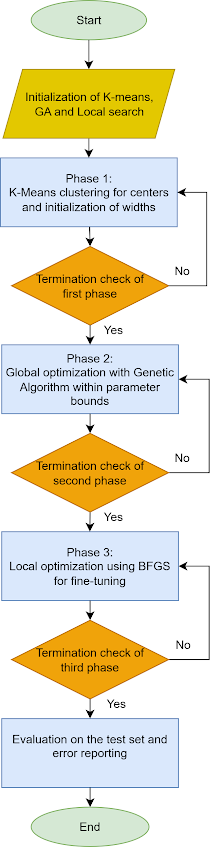
\includegraphics[scale=0.5]{overall_flowchart}
\par\end{centering}
\caption{Summary flowchart of the proposed method.\label{fig:summary}}

\end{figure}


\section{Results\label{sec:Results}}

The proposed method was validated using a series of classification
and regression datasets, obtained from the following online databases:
\begin{enumerate}
\item The UCI database, \url{https://archive.ics.uci.edu/}(accessed on
29 August 2025)\citep{uci}
\item The Keel website, \url{https://sci2s.ugr.es/keel/datasets.php}(accessed
on 29 August 2025)\citep{Keel}.
\item The Statlib database \url{https://lib.stat.cmu.edu/datasets/index}(accessed
on 29 August 2025). 
\end{enumerate}

\subsection{Experimental datasets }

The following datasets were incorporated in the experiments conducted
in this work:
\begin{enumerate}
\item \textbf{Appendictis} that is a medical dataset \citep{appendicitis}. 
\item \textbf{Alcohol}, which is dataset regarding alcohol consumption \citep{alcohol}. 
\item \textbf{Australian}, which is a dataset produced from various bank
transactions \citep{australian}.
\item \textbf{Balance} dataset \citep{balance}, produced from various psychological
experiments.
\item \textbf{Cleveland}, a medical dataset which was discussed in a series
of papers \citep{cleveland1,cleveland2}. 
\item \textbf{Circular} dataset, which is an artificial dataset.
\item \textbf{Dermatology}, a medical dataset for dermatology problems \citep{dermatology}.
\item \textbf{Ecoli}, which is related to protein problems \citep{ecoli}.
\item \textbf{Hayes-roth} dataset \citep{hayes-roth}.
\item \textbf{Heart}, which is a dataset related to heart diseases \citep{heart}.
\item \textbf{HeartAttack}, which is a medical dataset for the detection
of heart diseases
\item \textbf{Housevotes}, a dataset which is related to the Congressional
voting in USA \citep{housevotes}.
\item \textbf{Ionosphere}, a dataset that contains measurements from the
ionosphere \citep{ion1,ion2}.
\item \textbf{Liverdisorder}, a medical dataset that was studied thoroughly
in a series of papers\citep{liver,liver1}.
\item \textbf{Lymography} \citep{lymography}.
\item \textbf{Mammographic}, which is a medical dataset used for the prediction
of breast cancer \citep{mammographic}.
\item \textbf{Parkinsons}, which is a medical dataset used for the detection
of Parkinson's disease \citep{parkinsons1,parkinsons2}.
\item \textbf{Pima}, which is a medical dataset for the detection of diabetes\citep{pima}.
\item \textbf{Popfailures}, a dataset related to experiments regarding climate
\citep{popfailures}.
\item \textbf{Regions2}, a medical dataset applied to liver problems \citep{regions2}.
\item \textbf{Saheart}, which is a medical dataset concerning heart diseases\citep{saheart}.
\item \textbf{Segment} dataset \citep{segment}.
\item \textbf{Statheart}, a medical dataset related to heart diseases.
\item \textbf{Spiral}, an artificial dataset with two classes.
\item \textbf{Student}, which is a dataset regarding experiments in schools
\citep{student}.
\item \textbf{Transfusion}, which is a medical dataset \citep{transfusion}.
\item \textbf{Wdbc}, which is a medical dataset regarding breast cancer
\citep{wdbc1,wdbc2}.
\item \textbf{Wine}, a dataset regarding measurements about the quality
of wines \citep{wine1,wine2}.
\item \textbf{EEG}, which is dataset regarding EEG recordings \citep{eeg1,eeg2}.
From this dataset the following cases were used: Z\_F\_S, ZO\_NF\_S,
ZONF\_S and Z\_O\_N\_F\_S.
\item \textbf{Zoo}, which is a dataset regarding animal classification \citep{zoo}
.
\end{enumerate}
Moreover a series of regression datasets was adopted in the conducted
experiments. The list with the regression datasets has as follows:
\begin{enumerate}
\item \textbf{Abalone}, which is a dataset about the age of abalones \citep{abalone}.
\item \textbf{Airfoil}, a dataset founded in NASA \citep{airfoil}.
\item \textbf{Auto}, a dataset related to the consumption of fuels from
cars.
\item \textbf{BK}, which is used to predict the points scored in basketball
games. 
\item \textbf{BL}, a dataset that contains measurements from electricity
experiments.
\item \textbf{Baseball}, which is a dataset used to predict the income of
baseball players.
\item \textbf{Concrete}, which is a civil engineering dataset \citep{concrete}.
\item \textbf{DEE}, a dataset that is used to predict the price of electricity.
\item \textbf{FA} dataset, related to fat measurements. 
\item \textbf{Friedman}, which is an artificial dataset\citep{friedman}.
\item \textbf{FY, }which is a dataset regarding the longevity of fruit flies. 
\item \textbf{HO}, a dataset located in the STATLIB repository.
\item \textbf{Housing}, regarding the price of houses \citep{housing}.
\item \textbf{Laser}, which contains measurements from various physics experiments.
\item \textbf{LW}, a dataset regarding the weight of babes.
\item \textbf{Mortgage}, a dataset that contains measurements from the economy
of USA.
\item \textbf{PL} dataset, located in the STALIB repository.
\item \textbf{Plastic}, a dataset regarding problems occurred with the pressure
on plastics.
\item \textbf{Quake}, a dataset regarding the measurements of earthquakes.
\item \textbf{SN}, a dataset related to trellising and pruning.
\item \textbf{Stock}, which is a dataset regarding stocks.
\item \textbf{Treasury}, a dataset that contains measurements from the economy
of USA.
\end{enumerate}

\subsection{Experimental results }

The experiments were performed on a Debian Linux system with 128GB
of ram and the code was implemented in ANSI C++ using the OPTIMUS
optimization environment \citep{optimus}. For the validation of the
experiments the ten - fold cross validation technique was utilized.
For the classification datasets the average classification error,
calculated on the corresponding test set, is reported. This quantity
is expressed using the following equation:
\begin{equation}
E_{C}\left(N\left(\overrightarrow{x},\overrightarrow{w}\right)\right)=100\times\frac{\sum_{i=1}^{N}\left(\mbox{class}\left(N\left(\overrightarrow{x_{i}},\overrightarrow{w}\right)\right)-y_{i}\right)}{N}
\end{equation}
Where the set $T$ denotes the related test set and it is defined
as $T=\left(x_{i},y_{i}\right),\ i=1,\ldots,N$. Similarly, the average
regression is reported for the case of regression datasets and it
is expressed using the following equation:
\begin{equation}
E_{R}\left(N\left(\overrightarrow{x},\overrightarrow{w}\right)\right)=\frac{\sum_{i=1}^{N}\left(N\left(\overrightarrow{x_{i}},\overrightarrow{w}\right)-y_{i}\right)^{2}}{N}
\end{equation}
The values for the parameters of the proposed method are listed in
Table \ref{tab:settings}. 

\begin{table}[H]
\caption{The values for each parameter of the proposed method.\label{tab:settings}}

\centering{}%
\begin{tabular}{|c|c|c|}
\hline 
NAME & MEANING & VALUE\tabularnewline
\hline 
\hline 
$k$ & Number of radial functions & $10$\tabularnewline
\hline 
$F$ & Scaling factor & $2.0$\tabularnewline
\hline 
$B_{w}$ & Bound value for the weights & $10.0$\tabularnewline
\hline 
$N_{c}$ & Number of chromosomes & $500$\tabularnewline
\hline 
$N_{g}$ & Maximum number of generations & $200$\tabularnewline
\hline 
$p_{s}$ & Selection rate & $0.1$\tabularnewline
\hline 
$p_{m}$ & Mutation rate & $0.05$\tabularnewline
\hline 
\end{tabular}
\end{table}
 In the experimental tables the following notation is used:
\begin{enumerate}
\item The column DATASET represents the name of the objective problem.
\item The column BFGS represents the incorporation of the BFGS optimization
method \citep{bfgs} for the training of an artificial neural network
\citep{nn1,nn2} with 10 processing nodes.
\item The column ADAM represents the application of the Adam optimizer \citep{Adam,AdamNN}
to train a neural network with 10 hidden nodes.
\item The column RBF-KMEANS stands for the original training of an RBF network.
\item The column NEAT (NeuroEvolution of Augmenting Topologies) \citep{neat}
stands for the method NEAT incorporated in the training of neural
networks.
\item The column GENRBF stands method introduced in \citep{rbf_gen1} for
RBF training.
\item The column PROPOSED denotes the incorporation of the current work.
\item The row average denotes the average classification or regression error
for all datasets.
\end{enumerate}
Table \ref{tab:expClass} reports thirty-two classification datasets
and six learning methods: BFGS, ADAM, NEAT, RBF-KMEANS, GENRBF, and
the new proposed method. The entries are classification error rates;
lower values indicate better performance. The last row gives the mean
error for each method across all datasets. Based on these means, the
proposed method attains the lowest overall error, about 19.45\%. All
other methods exhibit substantially higher errors: GENRBF 34.89\%,
ADAM 33.73\%, BFGS 33.50\%, NEAT 32.77\%, and RBF-KMEANS 28.54\%.
Thus, on average, the proposed method nearly halves the error relative
to the alternatives. At the dataset level, the proposed approach often
delivers striking gains. For example, on Spiral it achieves only 13.26\%
error, whereas all other methods lie around 45--50\%. On Australian
it yields 22.67\% compared with 32--42\% for the others. Similarly,
on the challenging medical dataset Cleveland, it obtains 50.86\% while
the others exceed 67\%. Comparable advantages are observed on Heart,
HeartAttack, Statheart, Wine, and Z\_F\_S. There are, however, datasets
where the proposed method is not the best. On Hayes Roth and Zoo it
performs worse than GENRBF or RBF-KMEANS, and on Transfusion the results
are broadly similar to the other methods, with no clear advantage.
This indicates that although the method does not dominate in every
single problem, the overall trend clearly favors it. In summary, the
statistical picture suggests that the proposed method is, on average,
the most reliable and effective strategy, producing markedly lower
classification errors. While it lags behind certain alternatives on
a few datasets, its low mean error underscores a more general and
robust solution for classification tasks.

\begin{table}[H]
\caption{Experimental results on the classification datasets using the series
of machine learning methods used in this article. The number in cells
denote average classification error as measured on the corresponding
test set.\label{tab:expClass}}

\raggedright{}%
\begin{tabular}{|c|c|c|c|c|c|c|}
\hline 
\textbf{DATASET} & \textbf{BFGS} & \textbf{ADAM} & \textbf{NEAT} & \textbf{RBF-KMEANS} & \textbf{GENRBF} & \textbf{PROPOSED}\tabularnewline
\hline 
\hline 
Alcohol & 41.50\% & 57.78\% & 66.80\% & 49.38\% & 52.45\% & 28.57\%\tabularnewline
\hline 
Appendicitis & 18.00\% & 16.50\% & 17.20\% & 12.23\% & 16.83\% & 15.00\%\tabularnewline
\hline 
Australian & 38.13\% & 35.65\% & 31.98\% & 34.89\% & 41.79\% & 22.67\%\tabularnewline
\hline 
Balance & 8.64\% & 7.87\% & 23.14\% & 33.42\% & 38.02\% & 13.11\%\tabularnewline
\hline 
Cleveland & 77.55\% & 67.55\% & 53.44\% & 67.10\% & 67.47\% & 50.86\%\tabularnewline
\hline 
Circular & 6.08\% & 19.95\% & 35.18\% & 5.98\% & 21.43\% & 5.13\%\tabularnewline
\hline 
Dermatology & 52.92\% & 26.14\% & 32.43\% & 62.34\% & 61.46\% & 36.00\%\tabularnewline
\hline 
Hayes Roth & 37.33\% & 59.70\% & 50.15\% & 64.36\% & 63.46\% & 38.31\%\tabularnewline
\hline 
Heart & 39.44\% & 38.53\% & 39.27\% & 31.20\% & 28.44\% & 16.07\%\tabularnewline
\hline 
HeartAttack & 46.67\% & 45.55\% & 32.34\% & 29.00\% & 40.48\% & 19.20\%\tabularnewline
\hline 
HouseVotes & 7.13\% & 7.48\% & 10.89\% & 6.13\% & 11.99\% & 3.65\%\tabularnewline
\hline 
Ionosphere & 15.29\% & 16.64\% & 19.67\% & 16.22\% & 19.83\% & 12.17\%\tabularnewline
\hline 
Liverdisorder & 42.59\% & 41.53\% & 30.67\% & 30.84\% & 36.97\% & 29.29\%\tabularnewline
\hline 
Lymography & 35.43\% & 29.26\% & 33.70\% & 25.50\% & 29.33\% & 24.36\%\tabularnewline
\hline 
Mammographic & 17.24\% & 46.25\% & 22.85\% & 21.38\% & 30.41\% & 17.79\%\tabularnewline
\hline 
Parkinsons & 27.58\% & 24.06\% & 18.56\% & 17.41\% & 33.81\% & 17.53\%\tabularnewline
\hline 
Pima & 35.59\% & 34.85\% & 34.51\% & 25.78\% & 27.83\% & 24.02\%\tabularnewline
\hline 
Popfailures & 5.24\% & 5.18\% & 7.05\% & 7.04\% & 7.08\% & 6.33\%\tabularnewline
\hline 
Regions2 & 36.28\% & 29.85\% & 33.23\% & 38.29\% & 39.98\% & 26.29\%\tabularnewline
\hline 
Saheart & 37.48\% & 34.04\% & 34.51\% & 32.19\% & 33.90\% & 28.50\%\tabularnewline
\hline 
Segment & 68.97\% & 49.75\% & 66.72\% & 59.68\% & 54.25\% & 45.00\%\tabularnewline
\hline 
Sonar & 25.85\% & 30.33\% & 34.10\% & 27.90\% & 37.13\% & 22.00\%\tabularnewline
\hline 
Spiral & 47.99\% & 48.90\% & 50.22\% & 44.87\% & 50.02\% & 13.26\%\tabularnewline
\hline 
Statheart & 39.65\% & 44.04\% & 44.36\% & 31.36\% & 42.94\% & 19.67\%\tabularnewline
\hline 
Student & 7.14\% & 5.13\% & 10.20\% & 5.49\% & 33.26\% & 5.23\%\tabularnewline
\hline 
Transfusion & 25.84\% & 25.68\% & 24.87\% & 26.41\% & 25.67\% & 26.04\%\tabularnewline
\hline 
Wdbc & 29.91\% & 35.35\% & 12.88\% & 7.27\% & 8.82\% & 5.54\%\tabularnewline
\hline 
Wine & 59.71\% & 29.40\% & 25.43\% & 31.41\% & 31.47\% & 9.47\%\tabularnewline
\hline 
Z\_F\_S & 39.37\% & 47.81\% & 38.41\% & 13.16\% & 23.37\% & 3.73\%\tabularnewline
\hline 
Z\_O\_N\_F\_S & 65.67\% & 78.79\% & 77.08\% & 48.70\% & 68.40\% & 41.00\%\tabularnewline
\hline 
ZO\_NF\_S & 43.04\% & 47.43\% & 43.75\% & 9.02\% & 22.18\% & 4.24\%\tabularnewline
\hline 
ZONF\_S & 15.62\% & 11.99\% & 5.44\% & 4.03\% & 17.41\% & 1.98\%\tabularnewline
\hline 
ZOO & 10.70\% & 14.13\% & 20.27\% & 21.93\% & 33.50\% & 9.80\%\tabularnewline
\hline 
\textbf{AVERAGE} & \textbf{33.50\%} & \textbf{33.73\%} & \textbf{32.77\%} & \textbf{28.54\%} & \textbf{34.89\%} & \textbf{19.45\%}\tabularnewline
\hline 
\end{tabular}
\end{table}
Table \ref{tab:expRegression} reports twenty-one regression datasets
and six machine-learning models: BFGS, ADAM, NEAT, RBF-KMEANS, GENRBF,
and the proposed method. The entries are absolute prediction errors;
smaller values indicate better model performance. The last row gives
the mean error for each method across all datasets. The analysis of
the means clearly shows that the proposed method attains the smallest
overall error, 5.87. The remaining methods have substantially higher
errors: BFGS 28.82, ADAM 21.39, NEAT 13.99, RBF-KMEANS 9.56, and GENRBF
13.38. This implies that the proposed approach greatly improves accuracy,
reducing the average error to nearly half of the best competing model
and far more compared with the classical BFGS and ADAM. At the dataset
level there are striking gaps. On Housing the proposed method records
an error of 15.36, whereas the other models range from 56 to 97. On
Stock the contrast is even stronger, with an error of only 1.44 while
others reach well above 300. Similarly, on Plastic the error drops
to 2.28, while the alternatives lie between 8 and 26. Comparable advantages
are observed on Mortgage, Treasury, Concrete, HO, Quake, and PL. There
are, however, a few cases where the proposed method is not the best;
for example, on FY and SN it shows slightly higher errors than some
competitors, though the differences are small, so no clear advantage
emerges there. Overall, the evidence indicates that the proposed method
is the most reliable and effective option on average, substantially
reducing regression error relative to all other techniques. Although
it does not lead on every dataset, the large reduction in mean error
and the strong results on several difficult problems demonstrate a
robust and broadly applicable solution for regression tasks.

\begin{table}[H]
\caption{Experimental results on the regression datasets using a series of
machine learning methods. Numbers in cells represent average regression
error as measured on the corresponding test set.\label{tab:expRegression}}

\raggedright{}%
\begin{tabular}{|c|c|c|c|c|c|c|}
\hline 
\textbf{DATASET} & \textbf{BFGS} & \textbf{ADAM} & \textbf{NEAT} & \textbf{RBF-KMEANS} & \textbf{GENRBF} & \textbf{PROPOSED}\tabularnewline
\hline 
Abalone & 5.69 & 4.30 & 9.88 & 7.37 & 9.98 & 6.12\tabularnewline
\hline 
Airfoil & 0.003 & 0.005 & 0.067 & 0.27 & 0.121 & 0.004\tabularnewline
\hline 
Auto & 60.97 & 70.84 & 56.06 & 17.87 & 16.78 & 8.81\tabularnewline
\hline 
Baseball & 119.63 & 77.90 & 100.39 & 93.02 & 98.91 & 88.05\tabularnewline
\hline 
BK & 0.28 & 0.03 & 0.15 & 0.02 & 0.023 & 0.022\tabularnewline
\hline 
BL & 2.55 & 0.28 & 0.05 & 0.013 & 0.005 & 0.0004\tabularnewline
\hline 
Concrete & 0.066 & 0.078 & 0.081 & 0.011 & 0.015 & 0.005\tabularnewline
\hline 
Dee & 2.36 & 0.630 & 1.512 & 0.17 & 0.25 & 0.15\tabularnewline
\hline 
Housing & 97.38 & 80.20 & 56.49 & 57.68 & 95.69 & 15.36\tabularnewline
\hline 
Friedman & 1.26 & 22.90 & 19.35 & 7.23 & 16.24 & 5.99\tabularnewline
\hline 
FA & 0.426 & 0.11 & 0.19 & 0.015 & 0.15 & 0.013\tabularnewline
\hline 
FY & 0.22 & 0.038 & 0.08 & 0.041 & 0.041 & 0.054\tabularnewline
\hline 
HO & 0.62 & 0.035 & 0.169 & 0.03 & 0.076 & 0.009\tabularnewline
\hline 
Laser & 0.015 & 0.03 & 0.084 & 0.03 & 0.075 & 0.016\tabularnewline
\hline 
Mortgage & 8.23 & 9.24 & 14.11 & 1.45 & 1.92 & 0.23\tabularnewline
\hline 
PL & 0.29 & 0.117 & 0.098 & 2.12 & 0.155 & 0.023\tabularnewline
\hline 
Plastic & 20.32 & 11.71 & 20.77 & 8.62 & 25.91 & 2.28\tabularnewline
\hline 
PY & 0.578 & 0.09 & 0.075 & 0.012 & 0.029 & 0.021\tabularnewline
\hline 
Quake & 0.42 & 0.06 & 0.298 & 0.07 & 0.79 & 0.036\tabularnewline
\hline 
SN & 0.40 & 0.026 & 0.174 & 0.027 & 0.027 & 0.026\tabularnewline
\hline 
Stock & 302.43 & 180.89 & 12.23 & 12.23 & 25.18 & 1.44\tabularnewline
\hline 
Treasury & 9.91 & 11.16 & 15.52 & 2.02 & 1.89 & 0.47\tabularnewline
\hline 
\textbf{AVERAGE} & \textbf{28.82} & \textbf{21.39} & \textbf{13.99} & \textbf{9.56} & \textbf{13.38} & \textbf{5.87}\tabularnewline
\hline 
\end{tabular}
\end{table}
Based on the executions carried out with scripts in the R language
concerning the processing of the experimental results on the classification
datasets, the significance levels of the $p$ parameter were calculated
in order to assess the statistical strength of the comparisons between
the proposed model and the alternative methods. In Figure \ref{fig:statClass}
these significance levels are illustrated according to the established
scale, where ns indicates no statistically significant difference
$\left(p>0.005\right)$, while the presence of one to four asterisks
denotes increasing statistical strength, from significant $\left(p<0.05\right)$
to very extremely significant $\left(p<0.0001\right)$. The results
show that in all comparisons of the proposed model with the other
methods, namely BFGS, ADAM, NEAT, RBF-KMEANS, and GENRBF, the significance
levels were found at the highest level with $p<0.0001$. This indicates
that the performance differences are not random but instead reflect
a very strong superiority of the proposed model over all the other
techniques examined.

\begin{figure}[H]
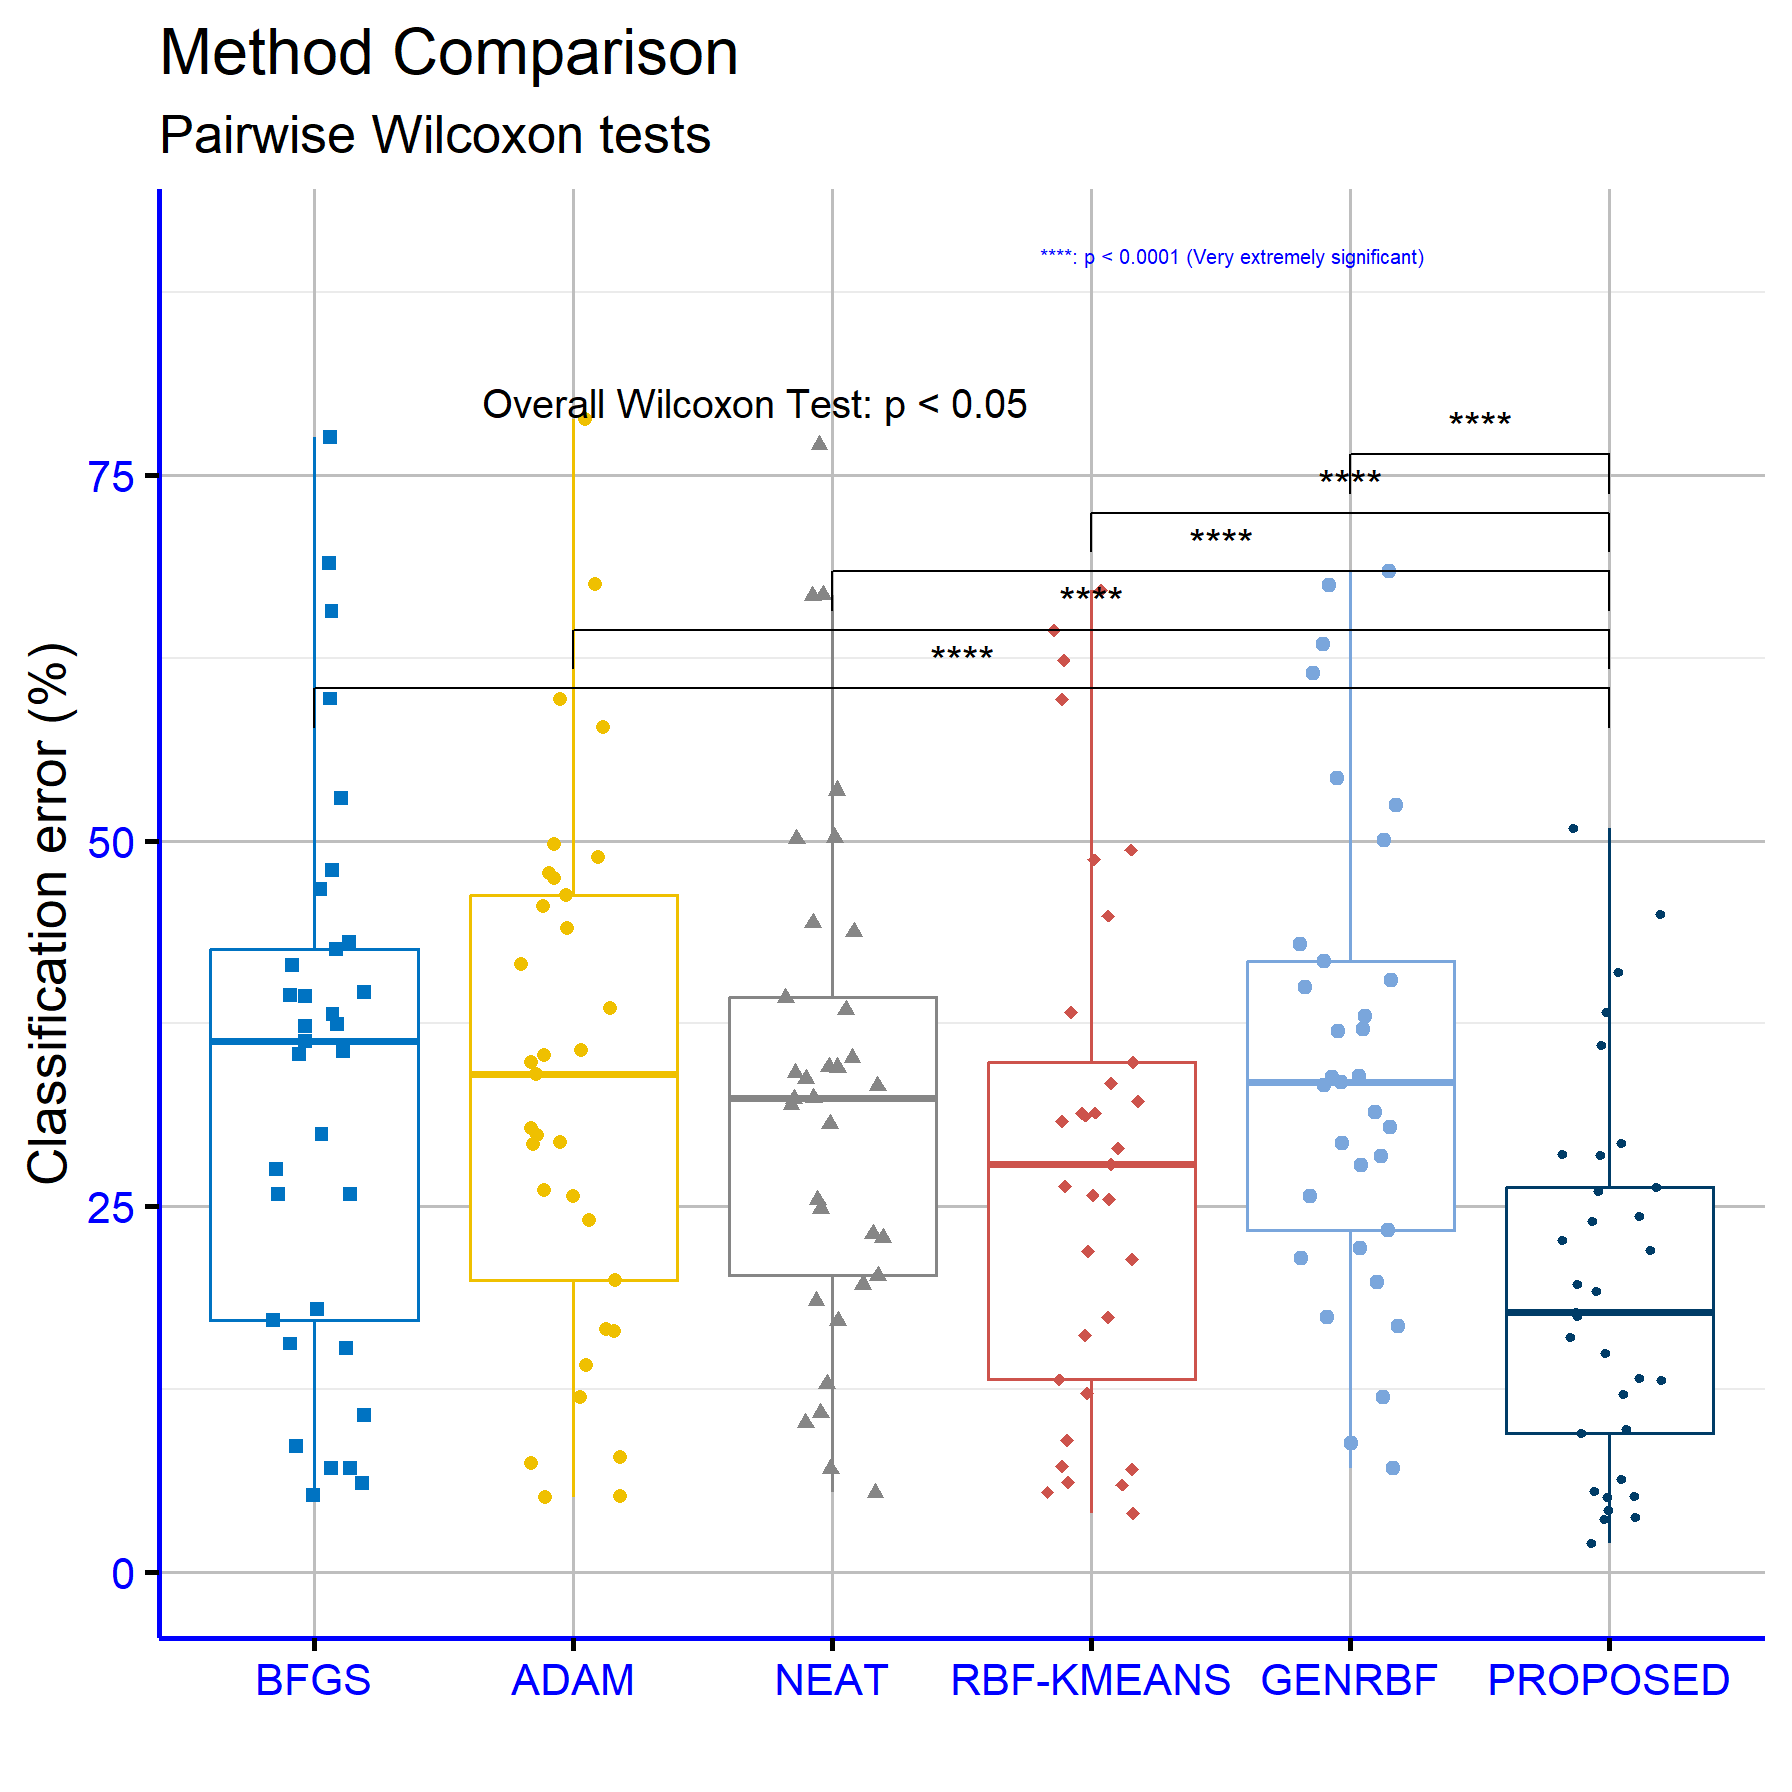
\includegraphics[scale=0.75]{stat1}

\caption{Statistical comparison of results obtained in the classification datasets
using a series of machine learning methods.\label{fig:statClass}}

\end{figure}
Similarly, for the regression datasets, the significance levels of
the $p$ parameter were computed to assess the statistical strength
of the comparisons between the proposed model and the other methods.
In Figure \ref{fig:statRegression}, the significance levels are illustrated
according to the established scale, where two asterisks correspond
to high statistical significance $\left(p<0.01\right)$ and four asterisks
indicate a very extremely significant difference $\left(p<0.0001\right)$.
The results show that, in comparison with the BFGS and ADAM models,
the proposed method achieves high statistical significance with $p<0.01$,
demonstrating that its superiority is not due to chance. Furthermore,
in all other comparisons, namely against NEAT, RBF-KMEANS, and GENRBF,
the significance levels reach the highest level with $p<0.0001$,
which highlights a very strong superiority of the proposed model over
the alternative regression methods examined.
\begin{figure}[H]
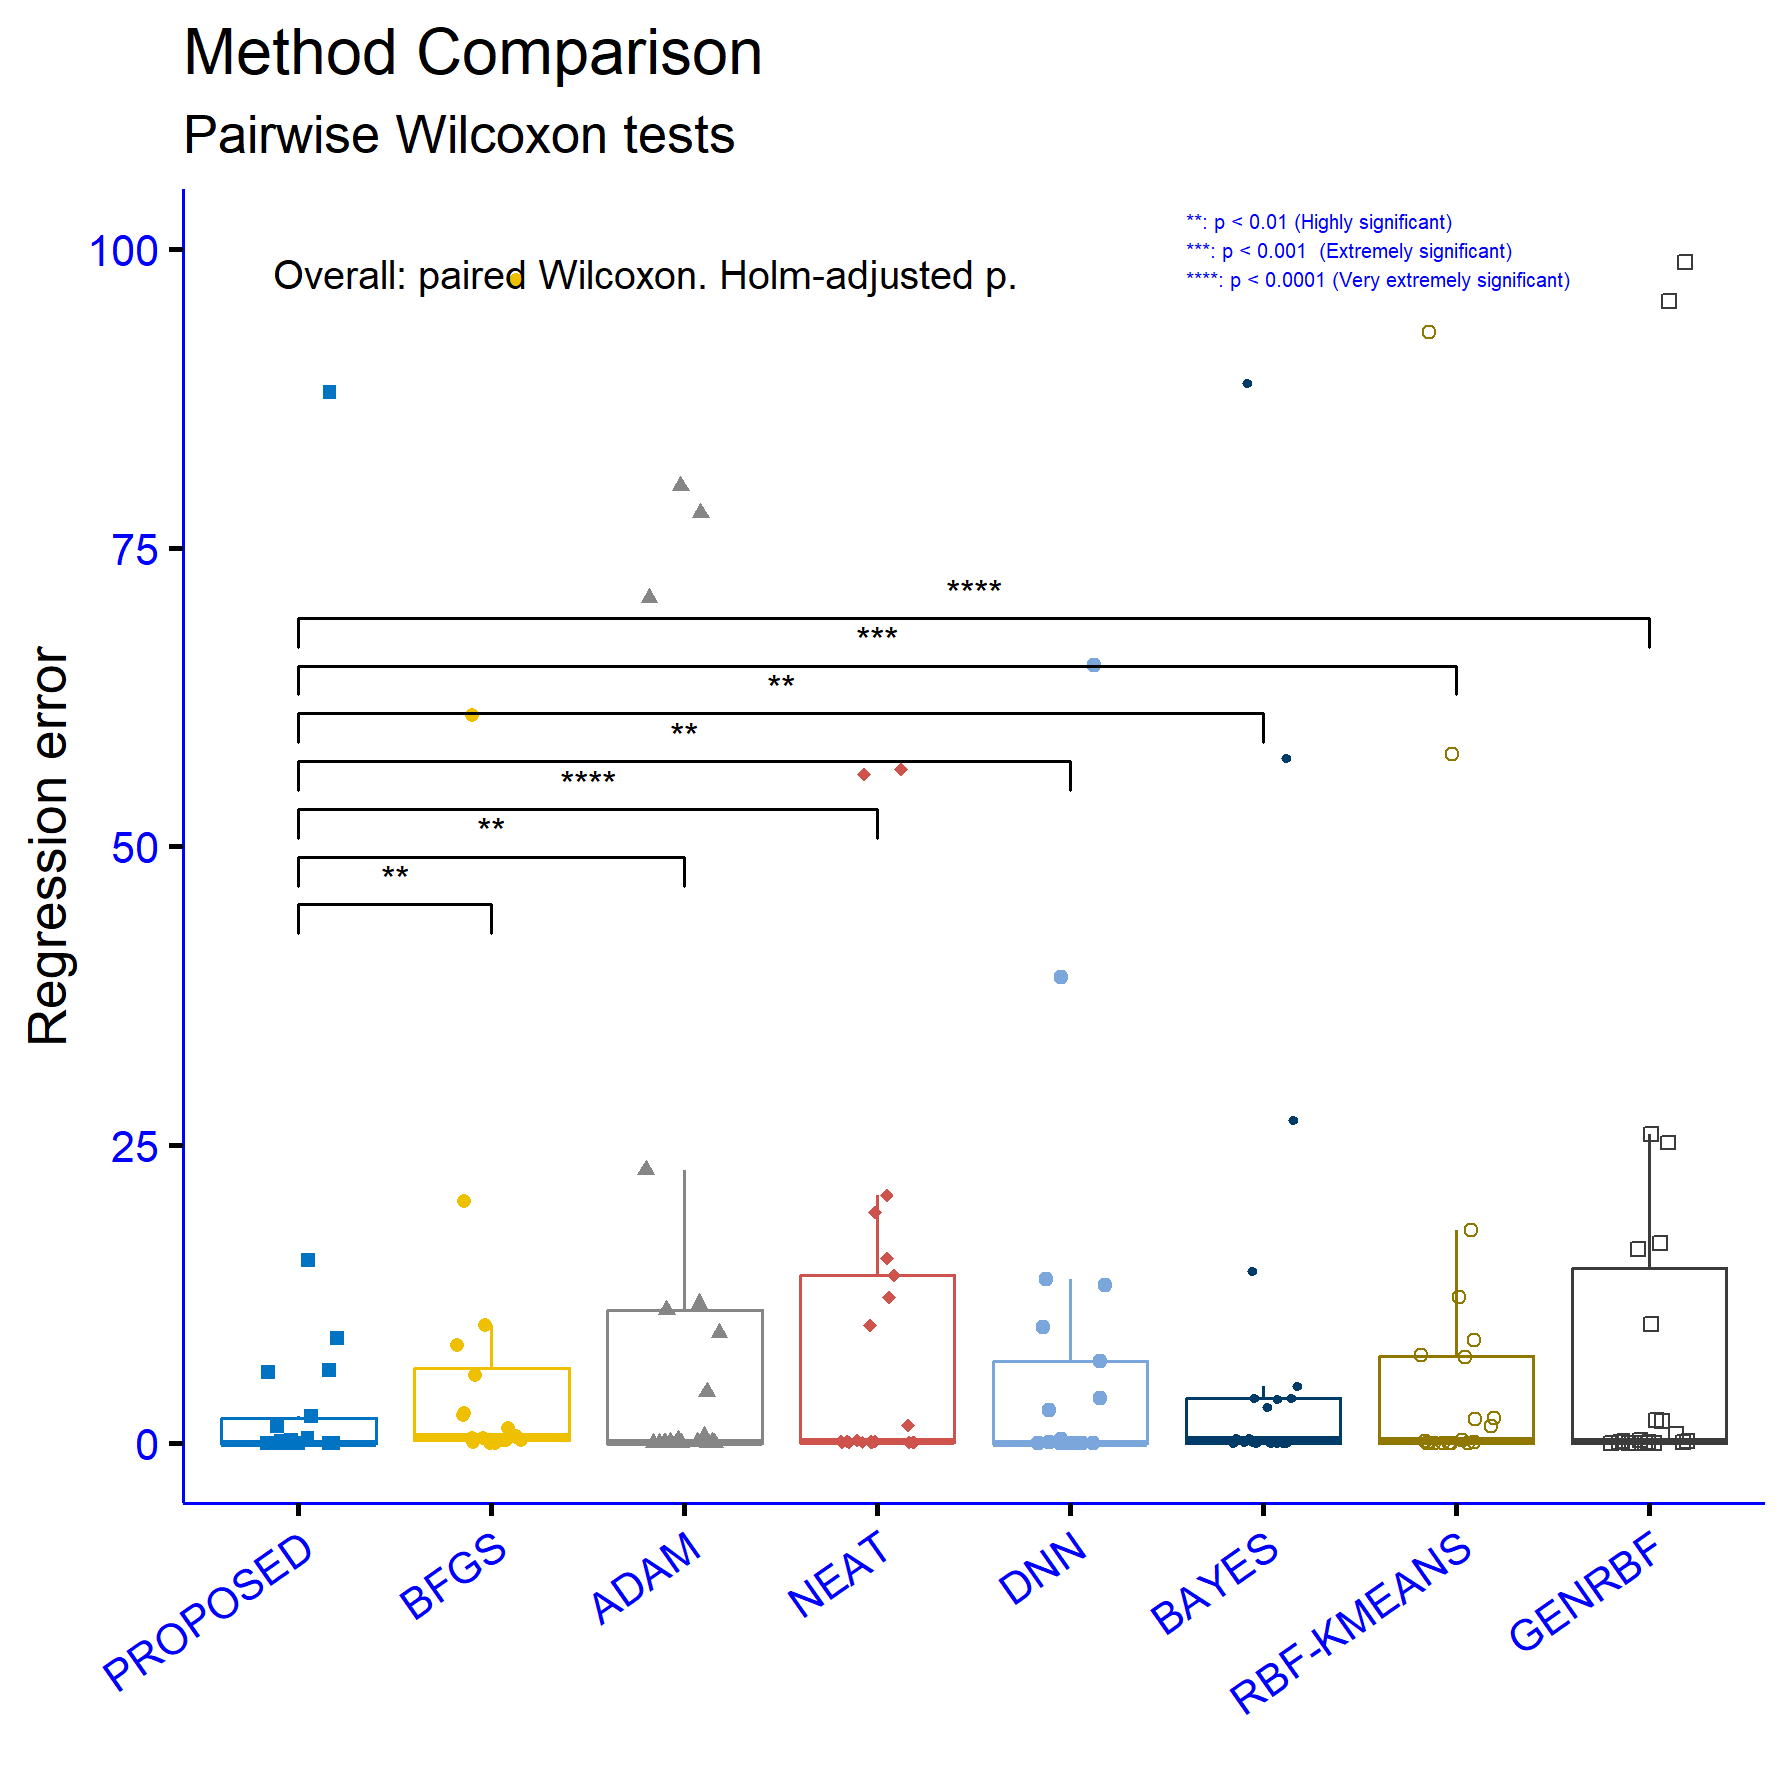
\includegraphics[scale=0.75]{stat2}

\caption{Statistical comparison of the obtained results in the regression datasets
using a variety of machine learning methods.\label{fig:statRegression}}

\end{figure}


\subsection{Experiments with different values of scale factor $F$ }

In order to determine the stability of the proposed technique when
its critical parameters change, a series of additional experiments
were conducted. In one of them, the stability of the technique was
studied with the change of the scale factor $F$. This factor controls
the width of the value interval for the network parameters and is
a multiple of the initial values estimated by the K-means method of
the first phase. In this series of experiments the value of $F$ was
altered in the range $[1,8]$. 

Table \ref{tab:expClassF} presents the effect of the scale factor
$F$ on the performance of the proposed machine learning model. The
parameter $F$ takes four different values, 1, 2, 4, and 8, and for
each dataset the classification error rate is reported. Analyzing
the mean values, it is observed that $F=2$ and $F=4$ achieve the
best overall performance, with average errors of 19.45\% and 18.53\%
respectively, compared to 20.99\% for $F=1$ and 18.60\% for $F=8$.
This indicates that selecting an intermediate value of the initialization
factor improves performance, reducing the error by about two percentage
points relative to the baseline case of $F=1$. At the individual
dataset level, interesting patterns emerge. For example, in Sonar
the error drops significantly from 32.90\% at $F=1$ to 18.75\% at
$F=4$, suggesting that the parameter $F$ strongly influences performance
in certain problems. In contrast, in Spiral increasing $F$ worsens
the results, as the error rises from 12.03\% at $F=1$ to 23.56\%
at $F=8$. Similarly, in the Australian dataset a gradual increase
of $F$ from 1 to 8 systematically improves performance, reducing
the error from 24.04\% to 20.59\%. Overall, the data show that the
effect of the scale factor is not uniform across all problems, but
the general trend indicates improvement when $F$ increases from 1
to 2 or 4. Choosing $F=4$ appears to yield the best mean result,
although the difference compared with $F=8$ is very small. Therefore,
it can be concluded that tuning this parameter plays an important
role in the stability and accuracy of the model, and that intermediate
values such as 4 constitute a good general choice.

\begin{table}[H]
\caption{Experimental results on the classification datasets using the proposed
method and a series of values for the critical parameter $F$.\label{tab:expClassF}}

\centering{}%
\begin{tabular}{|c|c|c|c|c|}
\hline 
\textbf{DATASET} & $F=1$ & \textbf{$F=2$} & $F=4$ & $F=8$\tabularnewline
\hline 
\hline 
Alcohol & 28.83\% & 28.57\% & 28.83\% & 30.09\%\tabularnewline
\hline 
Appendicitis & 14.60\% & 15.00\% & 14.40\% & 15.50\%\tabularnewline
\hline 
Australian & 24.04\% & 22.67\% & 21.52\% & 20.59\%\tabularnewline
\hline 
Balance & 21.03\% & 13.11\% & 11.87\% & 11.44\%\tabularnewline
\hline 
Cleveland & 50.45\% & 50.86\% & 51.59\% & 50.90\%\tabularnewline
\hline 
Circular & 4.13\% & 5.13\% & 3.67\% & 3.49\%\tabularnewline
\hline 
Dermatology & 38.34\% & 36.00\% & 35.83\% & 34.97\%\tabularnewline
\hline 
Hayes Roth & 51.85\% & 38.31\% & 32.62\% & 33.92\%\tabularnewline
\hline 
Heart & 17.26\% & 16.07\% & 15.63\% & 15.30\%\tabularnewline
\hline 
HeartAttack & 22.07\% & 19.20\% & 19.30\% & 19.07\%\tabularnewline
\hline 
HouseVotes & 4.13\% & 3.65\% & 3.39\% & 4.81\%\tabularnewline
\hline 
Ionosphere & 14.69\% & 12.17\% & 8.83\% & 7.51\%\tabularnewline
\hline 
Liverdisorder & 29.35\% & 29.29\% & 28.53\% & 29.23\%\tabularnewline
\hline 
Lymography & 26.86\% & 24.36\% & 18.07\% & 19.86\%\tabularnewline
\hline 
Mammographic & 18.21\% & 17.79\% & 16.75\% & 17.05\%\tabularnewline
\hline 
Parkinsons & 18.32\% & 17.53\% & 15.68\% & 14.05\%\tabularnewline
\hline 
Pima & 23.53\% & 24.02\% & 23.72\% & 23.26\%\tabularnewline
\hline 
Popfailures & 7.83\% & 6.33\% & 5.15\% & 4.69\%\tabularnewline
\hline 
Regions2 & 26.27\% & 26.29\% & 26.15\% & 25.73\%\tabularnewline
\hline 
Saheart & 29.24\% & 28.50\% & 28.74\% & 29.41\%\tabularnewline
\hline 
Segment & 45.08\% & 45.00\% & 42.14\% & 42.10\%\tabularnewline
\hline 
Sonar & 32.90\% & 22.00\% & 18.75\% & 18.05\%\tabularnewline
\hline 
Spiral & 12.03\% & 13.26\% & 16.66\% & 23.56\%\tabularnewline
\hline 
Statheart & 19.30\% & 19.67\% & 20.00\% & 19.44\%\tabularnewline
\hline 
Student & 6.33\% & 5.23\% & 5.10\% & 5.55\%\tabularnewline
\hline 
Transfusion & 25.54\% & 26.04\% & 25.66\% & 24.42\%\tabularnewline
\hline 
Wdbc & 4.86\% & 5.54\% & 5.75\% & 5.29\%\tabularnewline
\hline 
Wine & 12.18\% & 9.47\% & 8.59\% & 7.65\%\tabularnewline
\hline 
Z\_F\_S & 4.37\% & 3.73\% & 3.73\% & 3.37\%\tabularnewline
\hline 
Z\_O\_N\_F\_S & 39.80\% & 41.00\% & 40.04\% & 40.80\%\tabularnewline
\hline 
ZO\_NF\_S & 4.26\% & 4.24\% & 4.58\% & 3.78\%\tabularnewline
\hline 
ZONF\_S & 2.52\% & 1.98\% & 2.58\% & 1.96\%\tabularnewline
\hline 
ZOO & 12.40\% & 9.80\% & 7.60\% & 6.90\%\tabularnewline
\hline 
\textbf{AVERAGE} & \textbf{20.99\%} & \textbf{19.45\%} & \textbf{18.53\%} & \textbf{18.60\%}\tabularnewline
\hline 
\end{tabular}
\end{table}
Table \ref{tab:expRegressionF} shows the effect of the scale factor
$F$ on the performance of the proposed regression model. Based on
the mean errors, the best overall performance occurs at $F=4$ with
an average error of 5.68, while the values for $F=1,F=2$ and $F=8$
are 5.94, 5.87, and 5.78, respectively. The differences across the
four settings are not large, but they indicate that intermediate values
and especially $F=4$ tend to offer the best accuracy stability trade-off.
At the level of individual datasets, substantial variations are observed.
For Friedman the reduction is dramatic, with error dropping from 6.74
at $F=1$ to 1.41 at $F=8$, highlighting that proper tuning of $F$
can have a strong impact on performance. Laser shows a similarly large
improvement, from 0.027 at $F=1$ to just 0.0024 at $F=8$. Mortgage
also improves markedly, from $0.67$ at $F=1$ to 0.015 at $F=8$.
By contrast, in some datasets the value of $F$ has little practical
effect, such as Quake and HO, where errors remain nearly constant
regardless of F. There are also cases like Housing where increasing
$F$ degrades performance, with error rising from 14.64 at $F=1$
to 18.48 at $F=8$. Overall, the results indicate that the scale factor
$F$ has a significant but nonuniform influence on model performance.
In some datasets it sharply reduces error, while in others its impact
is negligible or even negative. Nevertheless, the aggregate picture
based on the mean errors suggests that $F=4$ and $F=8$ yield the
most reliable results, with $F=4$ being the preferred choice for
a general-purpose setting.
\begin{table}[H]
\caption{Experimental results on the regression datasets using the proposed
technique and a series of values for the parameter $F$.\label{tab:expRegressionF}}

\centering{}%
\begin{tabular}{|c|c|c|c|c|}
\hline 
\textbf{DATASET} & $F=1$ & \textbf{$F=2$} & $F=4$ & $F=8$\tabularnewline
\hline 
Abalone & 6.70 & 6.12 & 5.70 & 5.56\tabularnewline
\hline 
Airfoil & 0.004 & 0.004 & 0.004 & 0.004\tabularnewline
\hline 
Auto & 10.04 & 8.81 & 9.82 & 10.92\tabularnewline
\hline 
Baseball & 87.01 & 88.05 & 85.87 & 86.76\tabularnewline
\hline 
BK & 0.023 & 0.022 & 0.024 & 0.02\tabularnewline
\hline 
BL & 0.01 & 0.0004 & 0.0002 & 0.00007\tabularnewline
\hline 
Concrete & 0.008 & 0.005 & 0.005 & 0.006\tabularnewline
\hline 
Dee & 0.15 & 0.15 & 0.16 & 0.16\tabularnewline
\hline 
Housing & 14.64 & 15.36 & 17.34 & 18.48\tabularnewline
\hline 
Friedman & 6.74 & 5.99 & 2.06 & 1.41\tabularnewline
\hline 
FA & 0.012 & 0.013 & 0.012 & 0.013\tabularnewline
\hline 
FY & 0.055 & 0.054 & 0.054 & 0.053\tabularnewline
\hline 
HO & 0.009 & 0.009 & 0.01 & 0.009\tabularnewline
\hline 
Laser & 0.027 & 0.016 & 0.005 & 0.0024\tabularnewline
\hline 
Mortgage & 0.67 & 0.23 & 0.035 & 0.015\tabularnewline
\hline 
PL & 0.023 & 0.023 & 0.023 & 0.022\tabularnewline
\hline 
Plastic & 2.32 & 2.28 & 2.26 & 2.22\tabularnewline
\hline 
PY & 0.019 & 0.021 & 0.013 & 0.011\tabularnewline
\hline 
Quake & 0.036 & 0.036 & 0.036 & 0.036\tabularnewline
\hline 
SN & 0.024 & 0.026 & 0.025 & 0.024\tabularnewline
\hline 
Stock & 1.69 & 1.44 & 1.49 & 1.48\tabularnewline
\hline 
Treasury & 0.57 & 0.47 & 0.035 & 0.031\tabularnewline
\hline 
\textbf{AVERAGE} & \textbf{5.94} & \textbf{5.87} & \textbf{5.68} & \textbf{5.78}\tabularnewline
\hline 
\end{tabular}
\end{table}

In Figure \ref{fig:statClassF}, the significance levels are presented
for the comparisons between different values of the parameter $F$
in the proposed machine learning method based on the classification
datasets. The analysis shows that the comparison between $F=1$ and
$F=2$ results in high statistical significance with $p<0.01$, indicating
that the transition from the initial value to $F=2$ has a substantial
impact on performance. Similarly, the comparison between $F=2$ and
$F=4$ also shows high statistical significance with $p<0.01$, suggesting
that further increasing the parameter continues to positively affect
the results. However, the comparison between $F=4$ and $F=8$ is
characterized as not statistically significant, since $p>0.05$, which
means that increasing the parameter beyond $F=4$ does not bring a
meaningful difference in performance. Overall, the findings indicate
that smaller values of $F$ play a critical role in improving the
model, while increases beyond 4 do not lead to further statistically
significant improvements.

\begin{figure}[H]
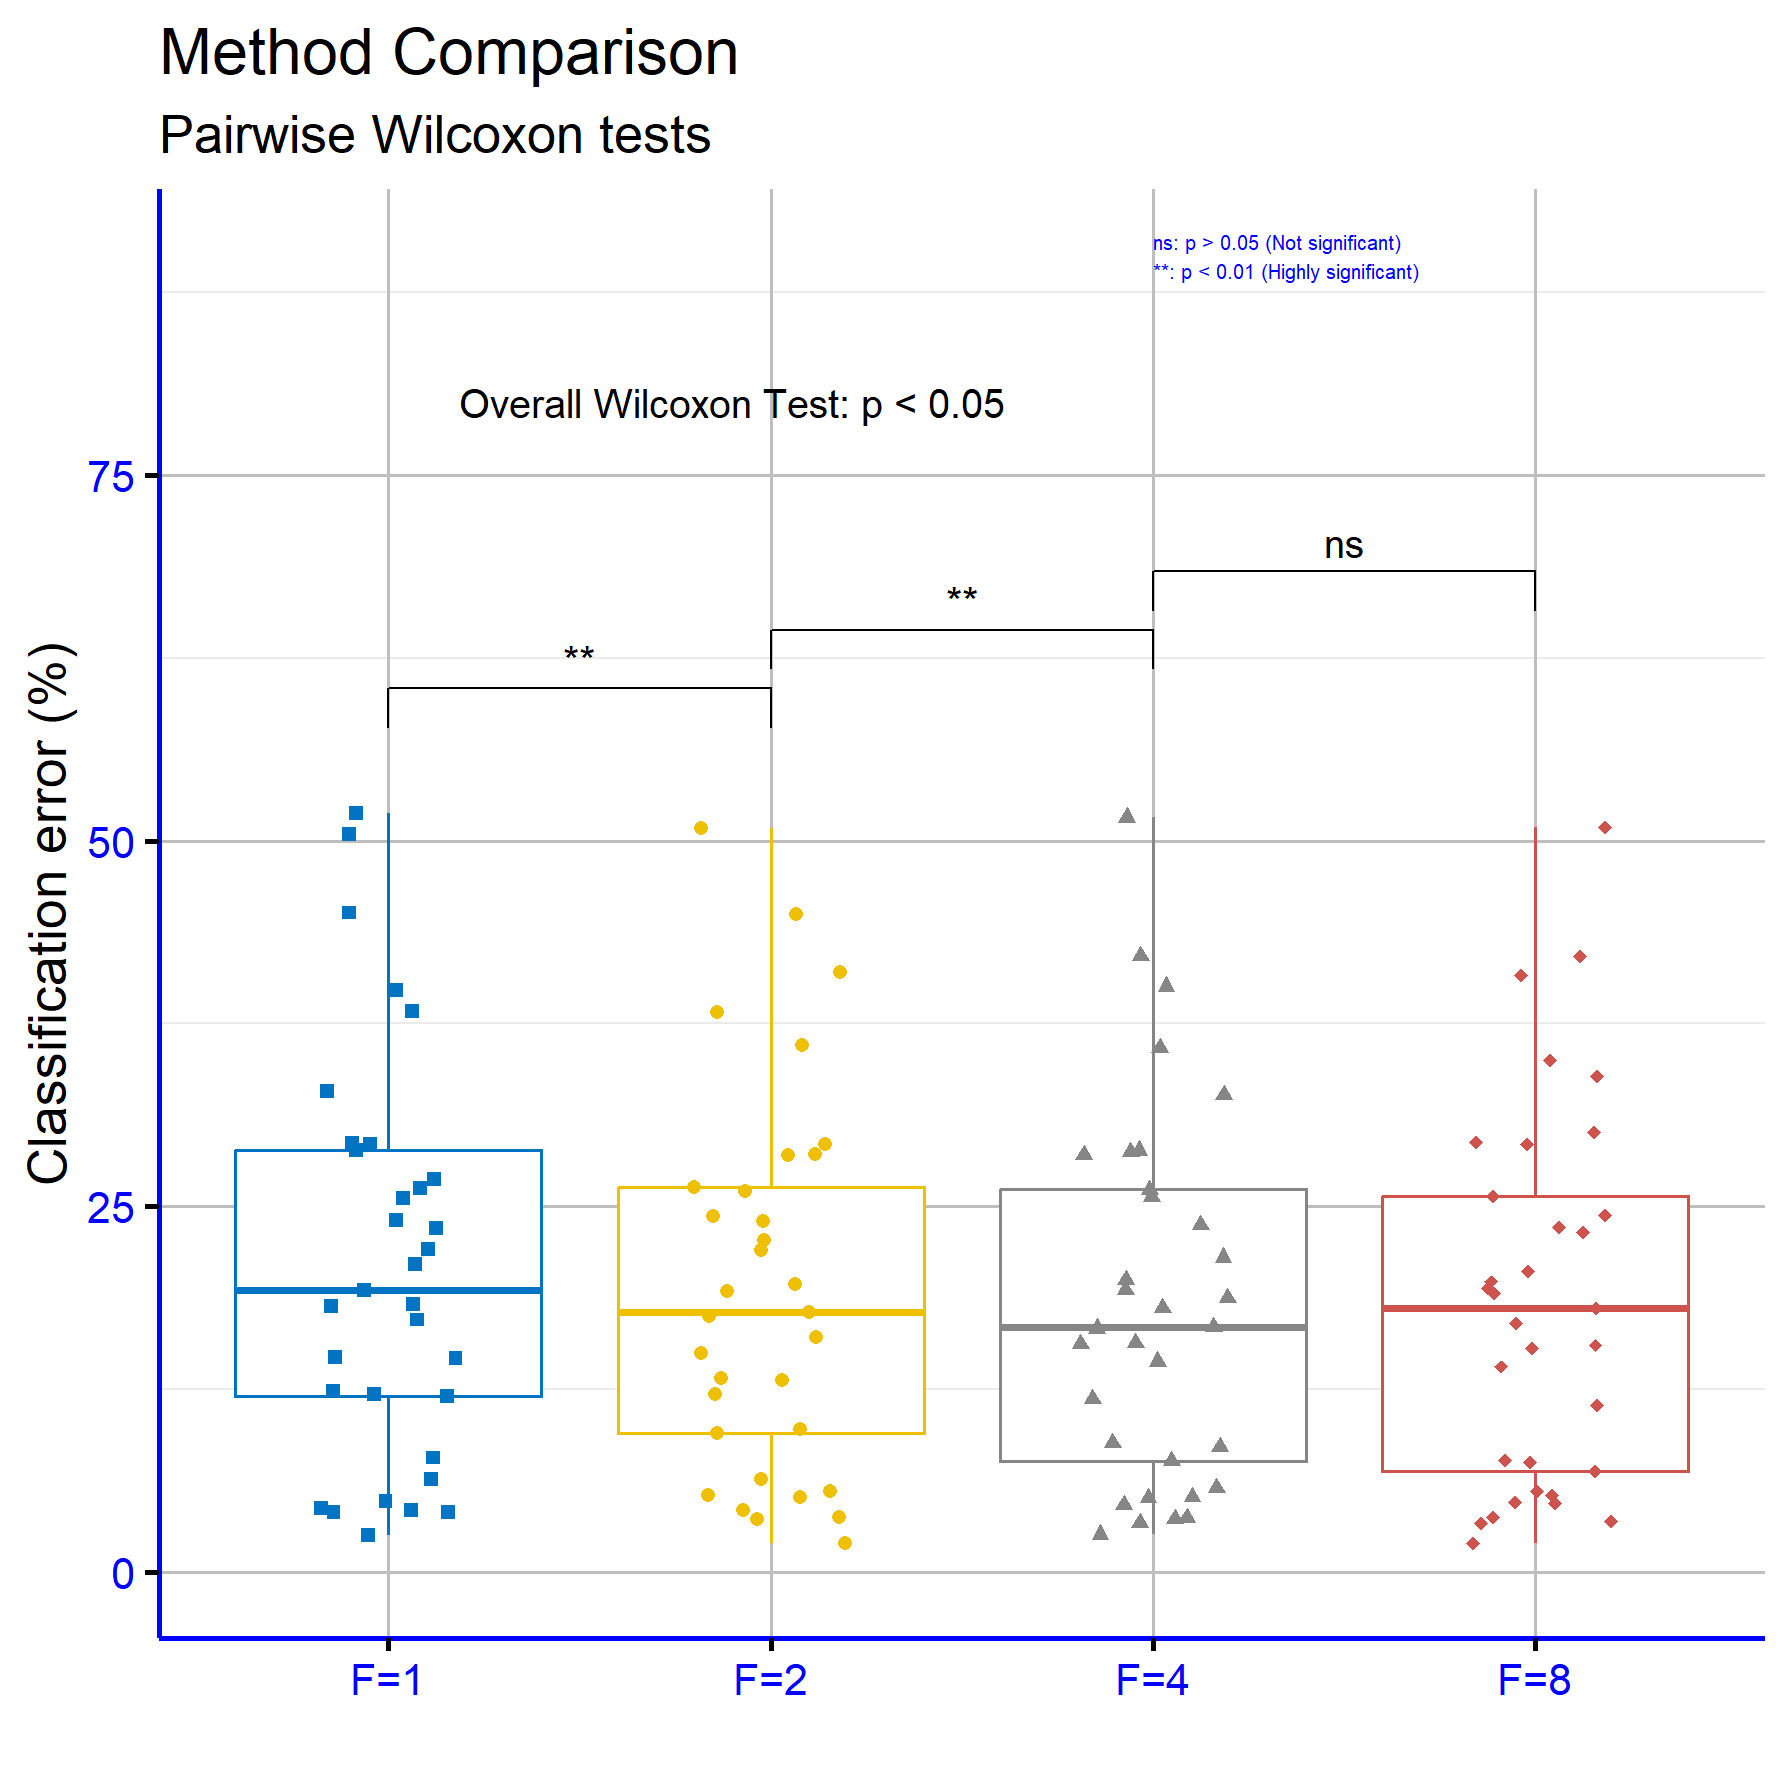
\includegraphics[scale=0.75]{stat3}

\caption{Statistical comparison for the obtained results on the classification
datasets using the proposed method and a series of values for the
scale parameter $F$.\label{fig:statClassF}}

\end{figure}
In Figure \ref{fig:statRegressionF}, the significance levels are
presented for the comparisons between different values of the parameter
F in the proposed method based on the regression datasets. The results
show that none of the comparisons $F=1$ vs $F=2$, $F=2$ vs $F=4$,
and $F=4$ vs $F=8$ exhibit statistically significant differences,
since in all cases $p>0.05$. This means that variations in the parameter
$F$ do not substantially affect the performance of the model in regression
problems. Therefore, it can be concluded that the choice of the $F$
value is not of critical importance for these datasets and that the
model remains stable regardless of the specific setting of this parameter.
\begin{figure}[H]
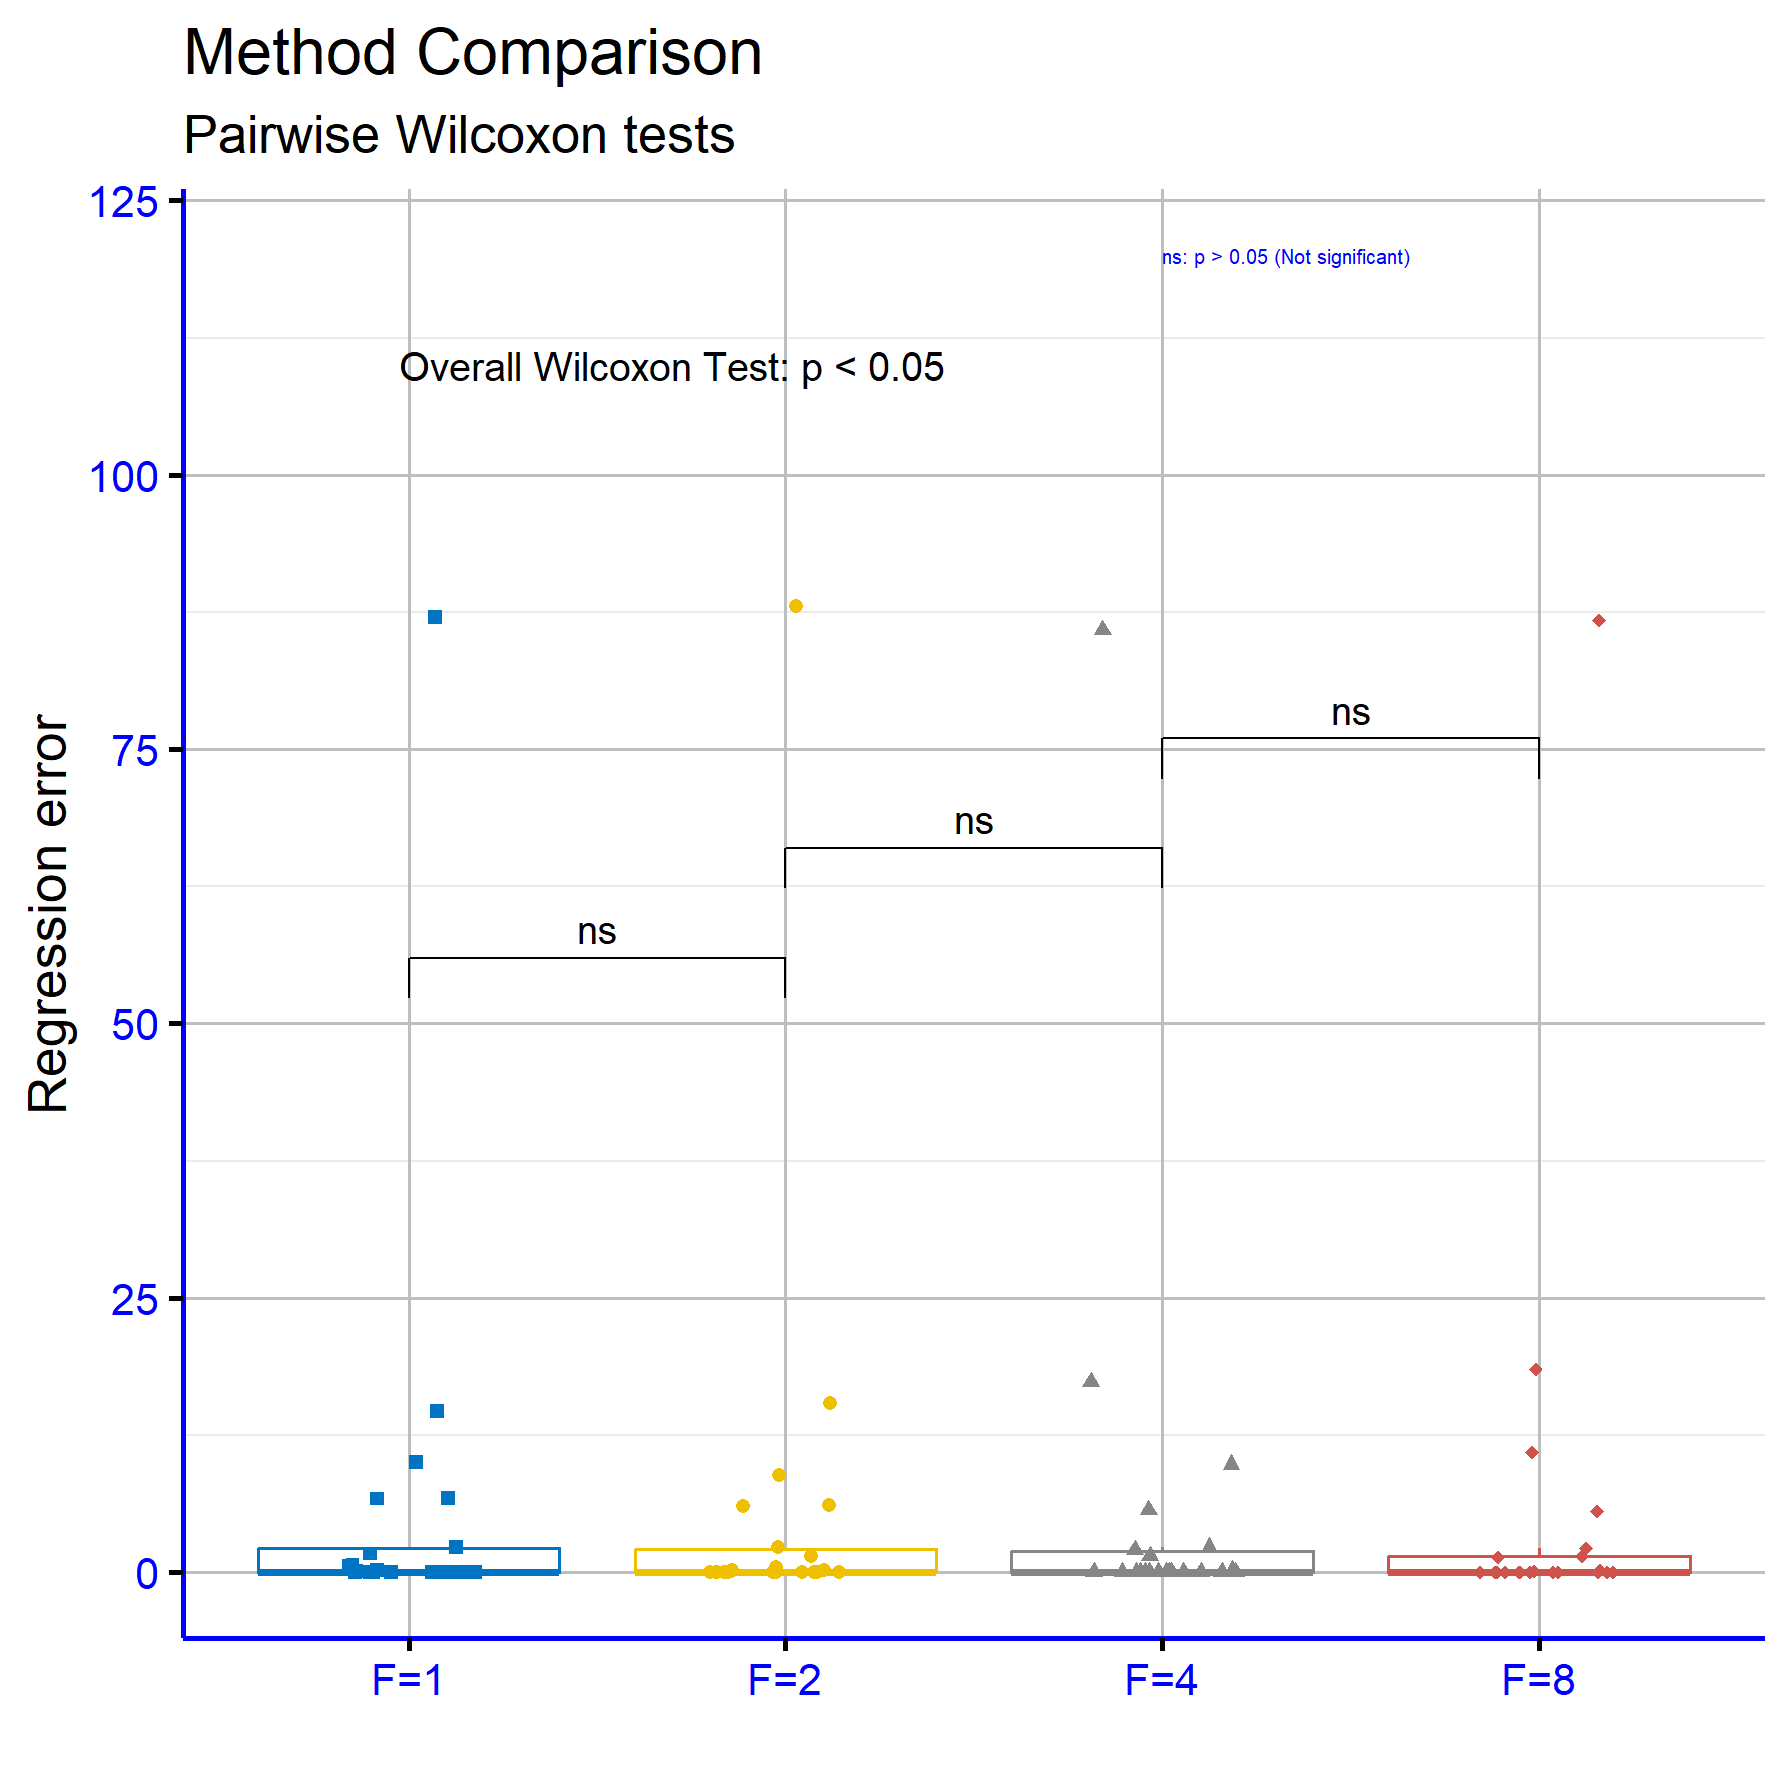
\includegraphics[scale=0.75]{stat4}

\caption{Statistical comparison for the experiments on the regression datasets,
using the proposed method and a series of values for the scale parameter
$F$.\label{fig:statRegressionF}}

\end{figure}


\subsection{Experiments with differential initialization methods for variances}

In another set of experiments, the stability of the proposed method
was checked, using a different way of calculating the range of values
of the $\sigma$ parameters of the radial functions. In this work,
the value of the variance produced by the K-means algorithm was used
as an initial estimate of the $\sigma$ parameters. This calculation
scheme is denoted as $\sigma_{1}$ in the following experimental tables.
In this additional set of experiments, two more techniques were used,
which will be denoted as $\sigma_{\mbox{avg}}$ and $\sigma_{\mbox{max}}$
in the following tables. In the $\sigma_{\mbox{avg}}$ the following
calculation is performed:
\begin{equation}
\sigma_{\mbox{avg}}=\frac{1}{k}\sum_{i=1}^{k}\sigma_{i}\label{eq:sigma_avg}
\end{equation}
Subsequently $\sigma_{\mbox{avg}}$ is used to determine the range
of values of the $\sigma$ parameters of the radial functions of the
network. In the $\sigma_{\mbox{avg}}$ the following quantity is calculated:
\begin{equation}
\sigma_{\mbox{max}}=\max\sigma_{i}\label{eq:sigma_max}
\end{equation}
Afterwards this quantity is used for the determination of the range
of values for the $\sigma$ parameters of the radial functions. 

Table \ref{tab:expClassSigma} presents the effect of three different
calculation techniques for the $\sigma$ parameters used in the radial
basis functions of the RBF model. The techniques are a fixed value
$\sigma_{1}$, the mean distance-based initialization $\left(\sigma_{\mbox{avg}}\right)$,
and the maximum distance--based initialization $\left(\sigma_{\mbox{max}}\right)$.
Based on the mean errors, the maximum-distance technique yields the
lowest overall error at 19.18\%. Very close is the mean-distance technique
at 19.27\%, while the simple $\sigma_{1}$ initialization has a slightly
higher error of 19.45\%. Although the differences among the three
approaches are small, the two adaptive methods $\left(\sigma_{\mbox{avg}}\ \mbox{and}\ \sigma_{\mbox{max}}\right)$
tend to produce marginally better overall performance. At the individual
dataset level, behaviors vary. For example, on Wine the $\sigma_{\mbox{max}}$
choice reduces error to 7.06\%, far below the 9.47\% obtained with
$\sigma_{1}$. On Dermatology, $\sigma_{1}$ performs better than
the other two, whereas on Segment the mean-based option is preferable.
In some cases the differences are minor e.g., Circular, Pima, and
Popfailures where all techniques are comparable; in others the choice
of technique materially affects performance, as in Transfusion, where
error drops from 26.04\% with $\sigma_{1}$ to about 22.78\% with
the other two methods. Overall, the statistical picture indicates
that no single technique dominates across all datasets. Nevertheless,
methods that adapt $\sigma$ to the geometry of the data $\left(\sigma_{\mbox{avg}}\ \mbox{and}\ \sigma_{\mbox{max}}\right)$
tend to yield more reliable and stable results, while the fixed value
lags slightly. The average differences are modest, but for certain
problems the choice can significantly impact final performance.

\begin{table}[H]
\caption{Experimental results on the classification datasets using the proposed
method and a series of techniques for the calculation of the quantities
$\sigma$ used in the radial functions.\label{tab:expClassSigma}}

\centering{}%
\begin{tabular}{|c|c|c|c|}
\hline 
\textbf{DATASET} & \textbf{$\sigma_{1}$} & $\sigma_{\mbox{avg}}$ & $\sigma_{\mbox{max}}$\tabularnewline
\hline 
\hline 
Alcohol & 28.57\% & 28.47\% & 26.17\%\tabularnewline
\hline 
Appendicitis & 15.00\% & 14.20\% & 15.70\%\tabularnewline
\hline 
Australian & 22.67\% & 25.14\% & 29.96\%\tabularnewline
\hline 
Balance & 13.11\% & 12.92\% & 12.23\%\tabularnewline
\hline 
Cleveland & 50.86\% & 51.76\% & 51.24\%\tabularnewline
\hline 
Circular & 5.13\% & 4.78\% & 4.45\%\tabularnewline
\hline 
Dermatology & 36.00\% & 37.54\% & 37.09\%\tabularnewline
\hline 
Hayes Roth & 38.31\% & 38.00\% & 35.69\%\tabularnewline
\hline 
Heart & 16.07\% & 16.52\% & 15.41\%\tabularnewline
\hline 
HeartAttack & 19.20\% & 19.70\% & 18.97\%\tabularnewline
\hline 
HouseVotes & 3.65\% & 3.31\% & 3.22\%\tabularnewline
\hline 
Ionosphere & 12.17\% & 13.00\% & 12.83\%\tabularnewline
\hline 
Liverdisorder & 29.29\% & 28.38\% & 27.77\%\tabularnewline
\hline 
Lymography & 24.36\% & 22.43\% & 23.50\%\tabularnewline
\hline 
Mammographic & 17.79\% & 17.28\% & 17.41\%\tabularnewline
\hline 
Parkinsons & 17.53\% & 14.74\% & 14.89\%\tabularnewline
\hline 
Pima & 24.02\% & 23.28\% & 23.91\%\tabularnewline
\hline 
Popfailures & 6.33\% & 6.37\% & 6.24\%\tabularnewline
\hline 
Regions2 & 26.29\% & 25.47\% & 25.61\%\tabularnewline
\hline 
Saheart & 28.50\% & 28.89\% & 28.28\%\tabularnewline
\hline 
Segment & 45.00\% & 43.65\% & 46.36\%\tabularnewline
\hline 
Sonar & 22.00\% & 21.90\% & 21.30\%\tabularnewline
\hline 
Spiral & 13.26\% & 13.73\% & 13.37\%\tabularnewline
\hline 
Statheart & 19.67\% & 20.15\% & 19.00\%\tabularnewline
\hline 
Student & 5.23\% & 5.58\% & 5.23\%\tabularnewline
\hline 
Transfusion & 26.04\% & 22.78\% & 22.79\%\tabularnewline
\hline 
Wdbc & 5.54\% & 5.22\% & 5.21\%\tabularnewline
\hline 
Wine & 9.47\% & 7.93\% & 7.06\%\tabularnewline
\hline 
Z\_F\_S & 3.73\% & 3.70\% & 3.73\%\tabularnewline
\hline 
Z\_O\_N\_F\_S & 41.00\% & 40.20\% & 41.12\%\tabularnewline
\hline 
ZO\_NF\_S & 4.24\% & 4.42\% & 4.84\%\tabularnewline
\hline 
ZONF\_S & 1.98\% & 1.92\% & 2.06\%\tabularnewline
\hline 
ZOO & 9.80\% & 12.50\% & 10.30\%\tabularnewline
\hline 
\textbf{AVERAGE} & \textbf{19.45\%} & \textbf{19.27\%} & \textbf{19.18\%}\tabularnewline
\hline 
\end{tabular}
\end{table}
Table \ref{tab:expRegressionSigma} presents the effect of three different
calculation techniques for the $\sigma$ parameters used in the radial
basis functions of RBF model. Based on the mean errors, the distance--average
method yields the lowest overall error at 5.81. Very close is the
fixed value $\sigma_{1}$ with a mean error of 5.87, while the maximum-distance
method shows a slightly higher mean error of 5.96. The difference
among the three methods is small, indicating that all can deliver
comparable performance at a general level, with a slight advantage
for the distance--average approach. At the level of individual datasets,
however, significant variations are observed. For example, in Mortgage
the $\sigma_{\mbox{max}}$ method reduces the error dramatically from
0.23 with $\sigma_{1}$ to 0.021, while $\sigma_{\mbox{avg}}$ also
provides a much better result with 0.041. In Treasury the improvement
is again substantial, as the error decreases from 0.47 with $\sigma_{1}$
to just 0.08 using $\sigma_{\mbox{max}}$. In Stock the reduction
is clear, from 1.44 to 1.23, while in Plastic both $\sigma_{\mbox{avg}}$
and $\sigma_{\mbox{max}}$ yield lower errors than $\sigma_{1}$.
On the other hand, in datasets such as Housing, the use of $\sigma_{\mbox{max}}$
worsens performance, increasing the error from 15.36 with $\sigma_{1}$
to 19.45. Similarly, in Auto and Baseball the lowest errors are obtained
with $\sigma_{1}$, whereas the alternative techniques result in slightly
worse performance. Overall, the results show that the choice of calculation
technique for $\sigma$ can significantly affect performance in certain
problems, while in others the difference is negligible. Although no
method consistently outperforms the others across all datasets, the
distance--average method appears slightly more reliable overall,
while the maximum-distance method can in some cases produce very large
improvements but in others lead to a degradation of performance.

\begin{table}[H]
\caption{Experimental results on the regression datasets using the proposed
method and a series of techniques for the calculation of the quantities
$\sigma$ used in the radial functions.\label{tab:expRegressionSigma}}

\centering{}%
\begin{tabular}{|c|c|c|c|}
\hline 
\textbf{DATASET} & \textbf{$\sigma_{1}$} & $\sigma_{\mbox{avg}}$ & $\sigma_{\mbox{max}}$\tabularnewline
\hline 
Abalone & 6.12 & 6.06 & 5.43\tabularnewline
\hline 
Airfoil & 0.004 & 0.003 & 0.003\tabularnewline
\hline 
Auto & 8.81 & 9.80 & 10.44\tabularnewline
\hline 
Baseball & 88.05 & 86.13 & 85.89\tabularnewline
\hline 
BK & 0.022 & 0.022 & 0.022\tabularnewline
\hline 
BL & 0.0004 & 0.008 & 0.0004\tabularnewline
\hline 
Concrete & 0.005 & 0.005 & 0.005\tabularnewline
\hline 
Dee & 0.15 & 0.16 & 0.16\tabularnewline
\hline 
Housing & 15.36 & 15.57 & 19.45\tabularnewline
\hline 
Friedman & 5.99 & 6.21 & 6.02\tabularnewline
\hline 
FA & 0.013 & 0.012 & 0.012\tabularnewline
\hline 
FY & 0.054 & 0.055 & 0.055\tabularnewline
\hline 
HO & 0.009 & 0.009 & 0.01\tabularnewline
\hline 
Laser & 0.016 & 0.018 & 0.011\tabularnewline
\hline 
Mortgage & 0.23 & 0.041 & 0.021\tabularnewline
\hline 
PL & 0.023 & 0.022 & 0.022\tabularnewline
\hline 
Plastic & 2.28 & 2.21 & 2.19\tabularnewline
\hline 
PY & 0.021 & 0.02 & 0.022\tabularnewline
\hline 
Quake & 0.036 & 0.036 & 0.036\tabularnewline
\hline 
SN & 0.026 & 0.026 & 0.025\tabularnewline
\hline 
Stock & 1.44 & 1.32 & 1.23\tabularnewline
\hline 
Treasury & 0.47 & 0.15 & 0.08\tabularnewline
\hline 
\textbf{AVERAGE} & \textbf{5.87} & \textbf{5.81} & \textbf{5.96}\tabularnewline
\hline 
\end{tabular}
\end{table}
In Figure \ref{fig:statClassSigma}, the significance levels are presented
for the comparisons of different computation techniques for the $\sigma$
parameters in the radial basis functions of the proposed machine learning
model, based on the classification datasets. The comparisons performed
$\sigma_{1}$ vs $\sigma_{\mbox{avg}}$, $\sigma_{1}$ vs $\sigma_{\mbox{max}}$,
and $\sigma_{\mbox{avg}}$ vs $\sigma_{\mbox{max}}$ did not show
any statistically significant differences, since in all cases $p>0.05$.
This indicates that the choice of compuation method for the $\sigma$
parameters does not substantially affect the performance of the model
on classification problems. Therefore, it can be concluded that the
model maintains stable performance regardless of which of the three
compuatation techniques is used.
\begin{figure}[H]
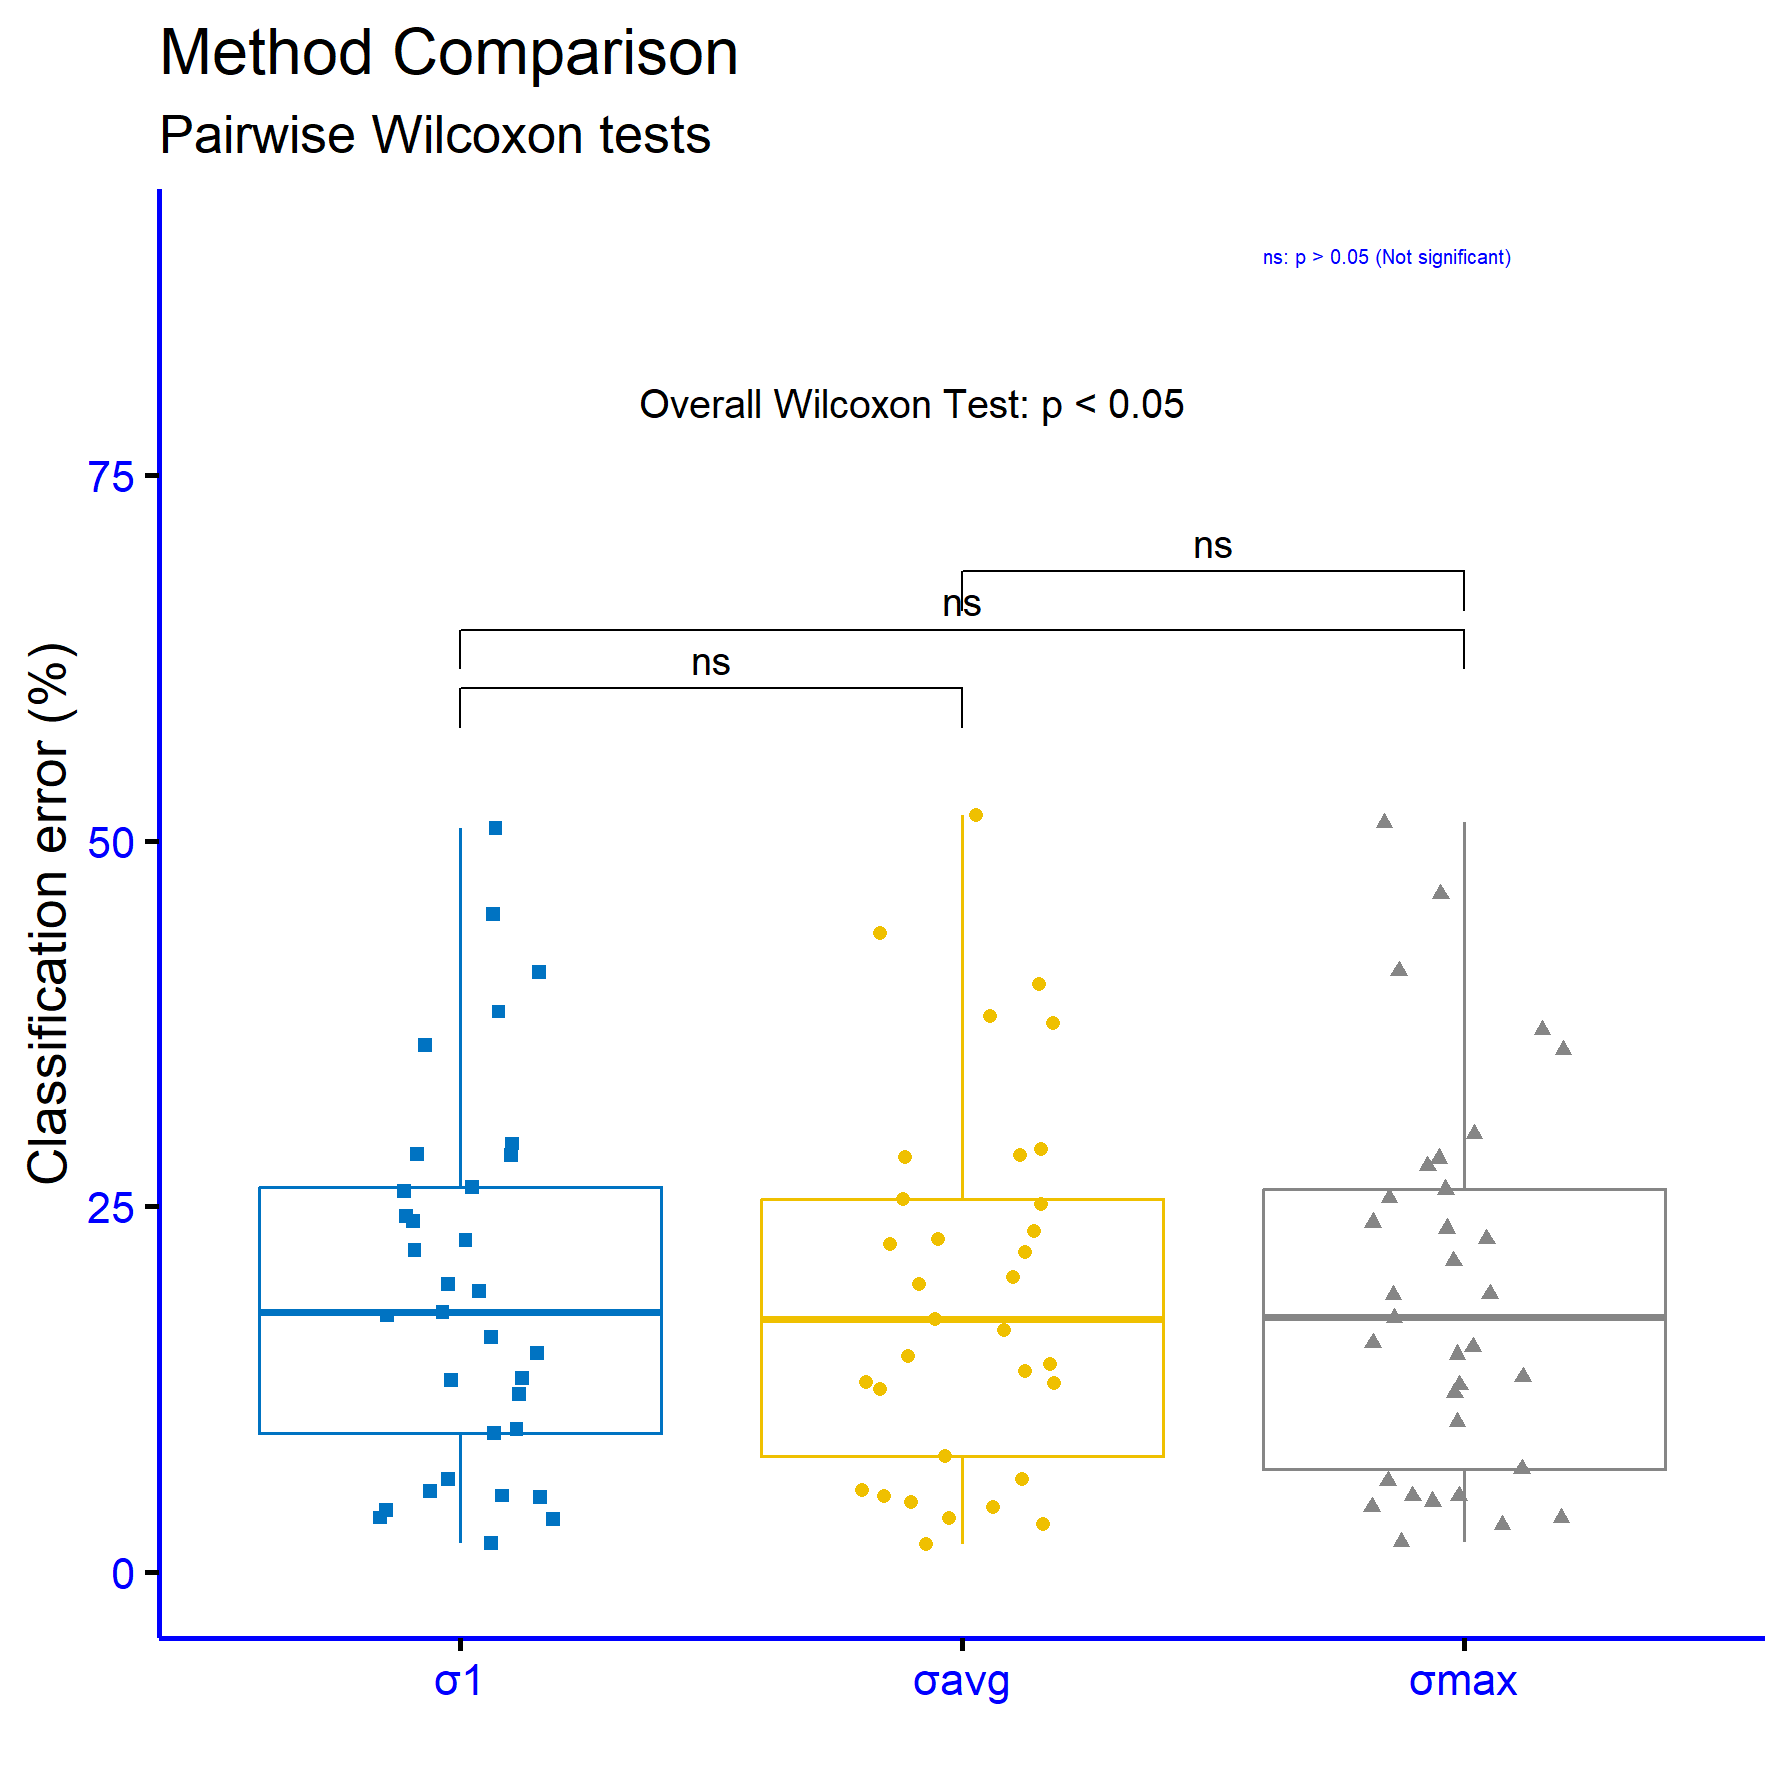
\includegraphics[scale=0.75]{stat5}

\caption{Statistical comparison of the obtained results on the classification
datasets, using the proposed method and a series of computation techniques
for the range of $\sigma$ values in the radial functions.\label{fig:statClassSigma}}

\end{figure}

In Figure \ref{fig:statRegressionSigma}, the significance levels
are presented for the comparisons of different computation techniques
for the $\sigma$ parameters in the radial basis functions of the
proposed machine learning model, based on the regression datasets.
The comparisons examined $\sigma_{1}$ vs $\sigma_{\mbox{avg}}$,
$\sigma_{1}$ vs $\sigma_{\mbox{max}}$, and $\sigma_{\mbox{avg}}$
vs $\sigma_{\mbox{max}}$ did not show any statistically significant
differences, since in all cases $p>0.05$. This means that the choice
of computation method for the $\sigma$ parameters does not have a
substantial impact on the performance of the model in regression problems.
Therefore, it can be concluded that the model demonstrates stable
and consistent behavior regardless of which initialization technique
is applied.

\begin{figure}[H]
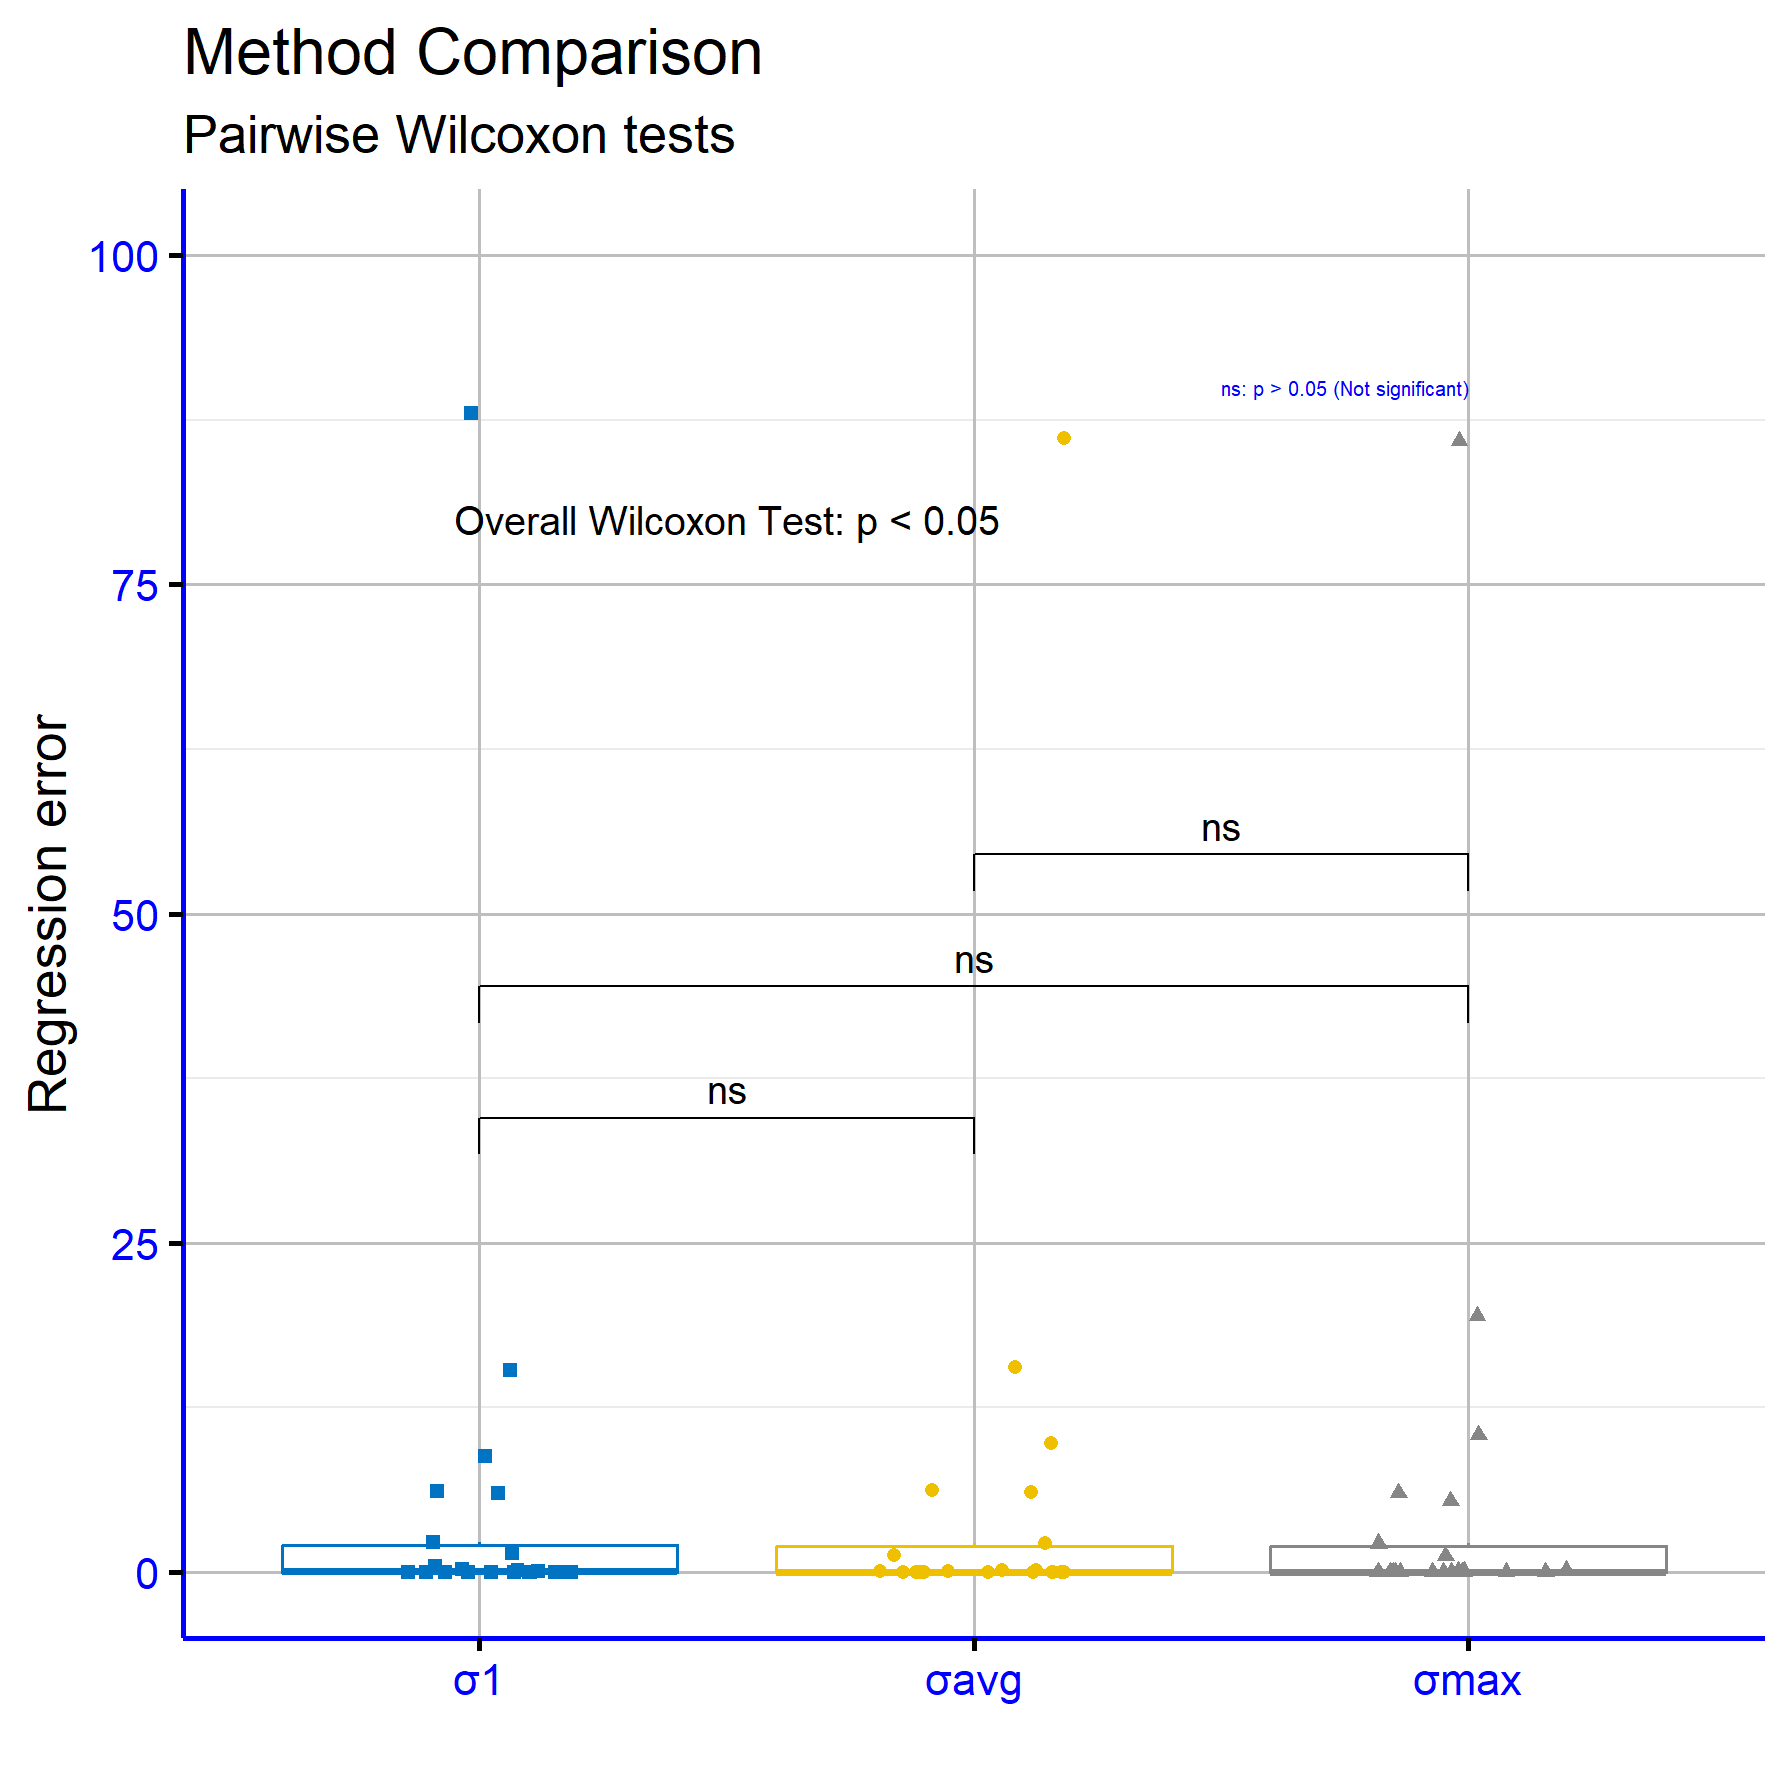
\includegraphics[scale=0.75]{stat6}

\caption{Statistical comparison of the obtained results on the regression datasets,
using the proposed method and a series of computation techniques for
the range of $\sigma$ values in the radial functions.\label{fig:statRegressionSigma}}

\end{figure}


\section{Conclusions\label{sec:Conclusions}}

The final experimental evidence shows that the three-phase RBF training
pipeline bound construction via K-means, global search with a GA inside
those bounds, and local refinement with BFGS yields robust gains across
heterogeneous classification and regression tasks. On classification,
it achieves the lowest mean error (19.45\%) with extremely significant
superiority over all baselines $\left(p<0.0001\right)$, on regression,
it attains the smallest mean absolute error (5.87), with $p<0.01$
against BFGS/ADAM and $p<0.0001$ against NEAT/RBF-KMEANS/GENRBF.
These results indicate that coupling broad exploration with constrained,
precise local tuning mitigates numerical instability and local minima,
providing reproducible performance improvements. 

Sensitivity analyses reveal that the scale factor $F$ materially
affects classification at small-to-intermediate settings ($F=1\rightarrow2$
and $F=2\rightarrow4$ are significant at $p<0.01$), with no meaningful
gain from $F=4$ to $F=8$, whereas for regression the $F$ comparisons
are not significant, highlighting methodological stability. Alternative
$\sigma$ computation methods $\left(\sigma_{1},\ \sigma_{\mbox{avg}},\ \sigma_{\mbox{max}}\right)$
differ only marginally on average and show no significant differences
in either task, reinforcing the method’s resilience to low-level design
choices. 

Automating architecture and hyperparameter adaptation is a natural
next step. Joint optimization of the number of RBF units, $F$, and
bounds via Bayesian optimization or meta-learning could reduce manual
tuning and improve generalization. Exploring alternative global optimizers
(e.g., DE, PSO, CMA-ES) or hybrid GA and Bayesian strategies may accelerate
convergence and enhance exploration, while in the final stage L-BFGS,
bound-aware variants, and stochastic formulations could benefit large-scale,
high-dimensional settings. A thorough ablation study to quantify each
phase’s contribution, along with broader post-hoc statistics, would
strengthen the evidence base. From a systems perspective, parallel/distributed
GA evaluations and GPU-accelerated RBF computations can materially
cut runtime. Finally, extending benchmarks to strong non-RBF baselines
and integrating the approach into AutoML pipelines together with analyses
of interpretability and predictive uncertainty will provide a more
complete picture of the method’s limits and potential.

\vspace{6pt}


\authorcontributions{V.C. and I.G.T. conducted the experiments, employing several datasets
and provided the comparative experiments. D.T. and V.C. performed
the statistical analysis and prepared the manuscript. All authors
have read and agreed to the published version of the manuscript.}

\funding{This research received no external funding.}

\institutionalreview{Not applicable.}

\informedconsent{Not applicable.}

\acknowledgments{This research has been financed by the European Union : Next Generation
EU through the Program Greece 2.0 National Recovery and Resilience
Plan , under the call RESEARCH -- CREATE -- INNOVATE, project name
“iCREW: Intelligent small craft simulator for advanced crew training
using Virtual Reality techniques\textquotedbl{} (project code:TAEDK-06195).}

\conflictsofinterest{The authors declare no conflicts of interest.}

\appendix

\begin{adjustwidth}{-\extralength}{0cm}{}

\reftitle{References}
\begin{thebibliography}{99}
\bibitem[(2006)]{physics_ml1} M. Mjahed, The use of clustering techniques
for the classification of high energy physics data, Nuclear Instruments
and Methods in Physics Research Section A: Accelerators, Spectrometers,
Detectors and Associated Equipment \textbf{559}, pp. 199-202, 2006.

\bibitem{physics_ml2}M Andrews, M Paulini, S Gleyzer, B Poczos, End-to-End
Event Classification of High-Energy Physics Data, Journal of Physics:
Conference Series \textbf{1085}, 2018.

\bibitem[(2006)]{astronomy_ml1}Viquar, M., Basak, S., Dasgupta, A.,
Agrawal, S., \& Saha, S. (2019). Machine learning in astronomy: A
case study in quasar-star classification. Emerging Technologies in
Data Mining and Information Security: Proceedings of IEMIS 2018, Volume
3, 827-836.

\bibitem[(2006)]{astronomy_ml2}Luo, S., Leung, A. P., Hui, C. Y.,
\& Li, K. L. (2020). An investigation on the factors affecting machine
learning classifications in gamma-ray astronomy. Monthly Notices of
the Royal Astronomical Society, 492(4), 5377-5390.

\bibitem[(2006)]{chemistry_ml1}P. He, C.J. Xu, Y.Z. Liang, K.T. Fang,
Improving the classification accuracy in chemistry via boosting technique,
Chemometrics and Intelligent Laboratory Systems 70, pp. 39-46, 2004.

\bibitem{chemistry_ml2}J.A. Aguiar, M.L. Gong, T.Tasdizen, Crystallographic
prediction from diffraction and chemistry data for higher throughput
classification using machine learning, Computational Materials Science
\textbf{173}, 109409, 2020.

\bibitem[(2006)]{med_ml1}S.S. Yadav, S.M. Jadhav, Deep convolutional
neural network based medical image classification for disease diagnosis.
J Big Data \textbf{6}, 113, 2019.

\bibitem{med_ml2}L. Qing, W. Linhong , D. Xuehai, A Novel Neural
Network-Based Method for Medical Text Classification, Future Internet
\textbf{11}, 255, 2019. 

\bibitem[(2006)]{econ_ml1}I. Kaastra, M. Boyd, Designing a neural
network for forecasting financial and economic time series, Neurocomputing
\textbf{10}, pp. 215-236, 1996.

\bibitem{econ_ml2}R. Hafezi, J. Shahrabi, E. Hadavandi, A bat-neural
network multi-agent system (BNNMAS) for stock price prediction: Case
study of DAX stock price, Applied Soft Computing \textbf{29}, pp.
196-210, 2015.

\bibitem{nn_image}M. Egmont-Petersen, D. de Ridder, H. Handels, Image
processing with neural networks---a review, Pattern Recognition \textbf{35},
pp. 2279-2301, 2002.

\bibitem{nn_timeseries}G.Peter Zhang, Time series forecasting using
a hybrid ARIMA and neural network model, Neurocomputing \textbf{50},
pp. 159-175, 2003.

\bibitem[(2006)]{rbfface}M.J. Er, S. Wu, J. Lu, H.L. Toh, Face recognition
with radial basis function (RBF) neural networks, IEEE Transactions
on Neural Networks \textbf{13}, pp. 697-710, 2002.

\bibitem[(2006)]{rbfde1}Nam Mai-Duy, Thanh Tran-Cong, Numerical solution
of differential equations using multiquadric radial basis function
networks, Neural Networks 14, pp. 185-199, 2001.

\bibitem{rbfde2}N. Mai‐Duy, Solving high order ordinary differential
equations with radial basis function networks. Int. J. Numer. Meth.
Engng. \textbf{62}, pp. 824-852, 2005.

\bibitem[(2006)]{rbfstock}Shen, W., Guo, X., Wu, C., \& Wu, D. (2011).
Forecasting stock indices using radial basis function neural networks
optimized by artificial fish swarm algorithm. Knowledge-Based Systems,
24(3), 378-385.

\bibitem[(2006)]{rbfrobotics1}R. -J. Lian, Adaptive Self-Organizing
Fuzzy Sliding-Mode Radial Basis-Function Neural-Network Controller
for Robotic Systems, IEEE Transactions on Industrial Electronics \textbf{61},
pp. 1493-1503, 2014.

\bibitem{rbfrobotics2}M. Vijay, D. Jena, Backstepping terminal sliding
mode control of robot manipulator using radial basis functional neural
networks. Computers \& Electrical Engineering \textbf{67}, pp. 690-707,
2018.

\bibitem[(2006)]{rbf_dos1}U. Ravale, N. Marathe, P. Padiya, Feature
Selection Based Hybrid Anomaly Intrusion Detection System Using K
Means and RBF Kernel Function, Procedia Computer Science \textbf{45},
pp. 428-435, 2015.

\bibitem{rbf_dos2}M. Lopez-Martin, A. Sanchez-Esguevillas, J. I.
Arribas, B. Carro, Network Intrusion Detection Based on Extended RBF
Neural Network With Offline Reinforcement Learning, IEEE Access \textbf{9},
pp. 153153-153170, 2021.

\bibitem[(2006)]{rbf_process}J. A. Leonard and M. A. Kramer, \textquotedbl Radial
basis function networks for classifying process faults,\textquotedbl{}
in IEEE Control Systems Magazine, vol. 11, no. 3, pp. 31-38, April
1991, doi: 10.1109/37.75576.

\bibitem[(2006)]{rbf_time}Ryad Zemouri and Daniel Racoceanu and Noureddine
Zerhouni, Recurrent radial basis function network for time-series
prediction, Engineering Applications of Artificial Intelligence 16,
pp. 453-463, 2003.

\bibitem[(2006)]{rbf_wind}G. Sideratos and N. Hatziargyriou, \textquotedbl Using
Radial Basis Neural Networks to Estimate Wind Power Production,\textquotedbl{}
2007 IEEE Power Engineering Society General Meeting, Tampa, FL, USA,
2007, pp. 1-7, doi: 10.1109/PES.2007.385812.

\bibitem[(2006)]{rbf_universal}J. Park and I. W. Sandberg, \textquotedbl Universal
Approximation Using Radial-Basis-Function Networks,\textquotedbl{}
in Neural Computation, vol. 3, no. 2, pp. 246-257, June 1991, doi:
10.1162/neco.1991.3.2.246. 

\bibitem[(2006)]{rbfinit1}L.I. Kuncheva, Initializing of an RBF network
by a genetic algorithm, Neurocomputing \textbf{14}, pp. 273-288, 1997.

\bibitem{rbfinit2}F. Ros, M. Pintore, A. Deman, J.R. Chrétien, Automatical
initialization of RBF neural networks, Chemometrics and Intelligent
Laboratory Systems \textbf{87}, pp. 26-32, 2007.

\bibitem{rbfinit3}D. Wang, X.J. Zeng, J.A. Keane, A clustering algorithm
for radial basis function neural network initialization, Neurocomputing
\textbf{77}, pp. 144-155, 2012.

\bibitem[(2006)]{rbfkernel}N. Benoudjit, M. Verleysen, On the Kernel
Widths in Radial-Basis Function Networks, Neural Processing Letters
\textbf{18}, pp. 139--154, 2003.

\bibitem[(2006)]{rbfprun1}E. Ricci, R. Perfetti, Improved pruning
strategy for radial basis function networks with dynamic decay adjustment,
Neurocomputing \textbf{69}, pp. 1728-1732, 2006.

\bibitem{rbfprun3}Guang-Bin Huang, P. Saratchandran and N. Sundararajan,
A generalized growing and pruning RBF (GGAP-RBF) neural network for
function approximation, IEEE Transactions on Neural Networks \textbf{16},
pp. 57-67, 2005.

\bibitem{rbfprun2}M. Bortman and M. Aladjem, A Growing and Pruning
Method for Radial Basis Function Networks, IEEE Transactions on Neural
Networks \textbf{20}, pp. 1039-1045, 2009.

\bibitem[(2006)]{rbfga1}Harpham, C., Dawson, C. W., \& Brown, M.
R. (2004). A review of genetic algorithms applied to training radial
basis function networks. Neural Computing \& Applications, 13, 193-201.

\bibitem[(2006)]{rbfga2}Sarimveis, H., Alexandridis, A., Mazarakis,
S., \& Bafas, G. (2004). A new algorithm for developing dynamic radial
basis function neural network models based on genetic algorithms.
Computers \& chemical engineering, 28(1-2), 209-217.

\bibitem[(2006)]{rbfpso1}Rani R, H. J., \& Victoire T, A. A. (2018).
Training radial basis function networks for wind speed prediction
using PSO enhanced differential search optimizer. PloS one, 13(5),
e0196871.

\bibitem[(2006)]{rbfpso2}Zhang, W., \& Wei, D. (2018). Prediction
for network traffic of radial basis function neural network model
based on improved particle swarm optimization algorithm. Neural Computing
and Applications, 29(4), 1143-1152.

\bibitem[(2006)]{rbfdiff1}Qasem, S. N., Shamsuddin, S. M., \& Zain,
A. M. (2012). Multi-objective hybrid evolutionary algorithms for radial
basis function neural network design. Knowledge-Based Systems, 27,
475-497.

\bibitem{rbfpar1}R. Yokota, L.A. Barba, M. G. Knepley, PetRBF ---
A parallel O(N) algorithm for radial basis function interpolation
with Gaussians, Computer Methods in Applied Mechanics and Engineering
\textbf{199}, pp. 1793-1804, 2010.

\bibitem{rbfpar2}C. Lu, N. Ma, Z. Wang, Fault detection for hydraulic
pump based on chaotic parallel RBF network, EURASIP J. Adv. Signal
Process. \textbf{2011}, 49, 2011.

\bibitem[(2006)]{kmeans}MacQueen, J.: Some methods for classification
and analysis of multivariate observations, in: Proceedings of the
fifth Berkeley symposium on mathematical statistics and probability,
Vol. 1, No. 14, pp. 281-297, 1967. 

\bibitem{kmeans-paterrn}Ali, H. H., \& Kadhum, L. E. (2017). K-means
clustering algorithm applications in data mining and pattern recognition.
International Journal of Science and Research (IJSR), 6(8), 1577-1584.

\bibitem{gen_kmeans}K. Krishna, M. Narasimha Murty, Genetic K-means
algorithm, IEEE Transactions on Systems, Man, and Cybernetics, Part
B (Cybernetics) \textbf{ 29}, pp. 433-439, 1999.

\bibitem{unsuper_kmeans}K. P. Sinaga, M. -S. Yang, Unsupervised K-Means
Clustering Algorithm, IEEE Access \textbf{8}, pp. 80716-80727, 2020. 

\bibitem{fixed_kmeans}M. Ay, L. Özbakır, S. Kulluk, B. Gülmez , G.Öztürk,
S. Özer, FC-Kmeans: Fixed-centered K-means algorithm, Expert Systems
with Applications \textbf{211}, 118656, 2023.

\bibitem{kmeans_review}E.U. Oti, M.O. Olusola, F.C. Eze, S.U. Enogwe,
Comprehensive review of K-Means clustering algorithms, Criterion \textbf{12},
pp. 22-23, 2021.

\bibitem{gen_app1}S.A. Grady, M.Y. Hussaini, M.M. Abdullah, Placement
of wind turbines using genetic algorithms, Renewable Energy \textbf{30},
pp. 259-270, 2005.

\bibitem{gen_app2}Prasad, T., Park, N., Multiobjective Genetic Algorithms
for Design of Water Distribution Networks, J. Water Resour. Plann.
Manage. \textbf{130}, pp. 73-82, 2004. 

\bibitem{gen_app3}Sung-Hwan Min, Jumin Lee, Ingoo Han, Hybrid genetic
algorithms and support vector machines for bankruptcy prediction,
Expert Systems with Applications \textbf{31}, pp. 652-660, 2006.

\bibitem{gen_app4}D. Whitley, T. Starkweather, C. Bogart, Genetic
algorithms and neural networks: Optimizing connections and connectivity,
Parallel Computing \textbf{14}, pp. 347-361, 1990.

\bibitem[(2004)]{pga1}Konfrst, Z. (2004, April). Parallel genetic
algorithms: Advances, computing trends, applications and perspectives.
In 18th International Parallel and Distributed Processing Symposium,
2004. Proceedings. (p. 162). IEEE.

\bibitem[(2004)]{pga2}Johar, F. M., Azmin, F. A., Suaidi, M. K.,
Shibghatullah, A. S., Ahmad, B. H., Salleh, S. N., ... \& Shukor,
M. M. (2013, November). A review of genetic algorithms and parallel
genetic algorithms on graphics processing unit (GPU). In 2013 IEEE
International Conference on Control System, Computing and Engineering
(pp. 264-269). IEEE.

\bibitem{kaelo}P. Kaelo, M.M. Ali, Integrated crossover rules in
real coded genetic algorithms, European Journal of Operational Research
\textbf{176}, pp. 60-76, 2007.

\bibitem[(2004)]{powell}M.J.D Powell, A Tolerant Algorithm for Linearly
Constrained Optimization Calculations, Mathematical Programming \textbf{45},
pp. 547-566, 1989. 

\bibitem[(2004)]{lbfgs}Liu, D. C., \& Nocedal, J. (1989). On the
limited memory BFGS method for large scale optimization. Mathematical
programming, 45(1), 503-528.

\bibitem[(2004)]{resbfgs}A. Mokhtari and A. Ribeiro, \textquotedbl RES:
Regularized Stochastic BFGS Algorithm,\textquotedbl{} in IEEE Transactions
on Signal Processing, vol. 62, no. 23, pp. 6089-6104, Dec.1, 2014,
doi: 10.1109/TSP.2014.2357775. 

\bibitem[(2004)]{conbfgs}Dai, Y. H. (2002). Convergence properties
of the BFGS algoritm. SIAM Journal on Optimization, 13(3), 693-701.

\bibitem[(1989)]{uci} M. Kelly, R. Longjohn, K. Nottingham, The UCI
Machine Learning Repository, \url{https://archive.ics.uci.edu}.

\bibitem{Keel}J. Alcalá-Fdez, A. Fernandez, J. Luengo, J. Derrac,
S. García, L. Sánchez, F. Herrera. KEEL Data-Mining Software Tool:
Data Set Repository, Integration of Algorithms and Experimental Analysis
Framework. Journal of Multiple-Valued Logic and Soft Computing 17,
pp. 255-287, 2011.

\bibitem{appendicitis}Weiss, Sholom M. and Kulikowski, Casimir A.,
Computer Systems That Learn: Classification and Prediction Methods
from Statistics, Neural Nets, Machine Learning, and Expert Systems,
Morgan Kaufmann Publishers Inc, 1991.

\bibitem[Tzimourta(2018)]{alcohol}Tzimourta, K.D.; Tsoulos, I.; Bilero,
I.T.; Tzallas, A.T.; Tsipouras, M.G.; Giannakeas, N. Direct Assessment
of Alcohol Consumption in Mental State Using Brain Computer Interfaces
and Grammatical Evolution. Inventions 2018, 3, 51.

\bibitem[Quinlan(2018)]{australian}J.R. Quinlan, Simplifying Decision
Trees. International Journal of Man-Machine Studies \textbf{27}, pp.
221-234, 1987. 

\bibitem{balance}T. Shultz, D. Mareschal, W. Schmidt, Modeling Cognitive
Development on Balance Scale Phenomena, Machine Learning \textbf{16},
pp. 59-88, 1994.

\bibitem[(2004)]{cleveland1}Z.H. Zhou,Y. Jiang, NeC4.5: neural ensemble
based C4.5,\textquotedbl{} in IEEE Transactions on Knowledge and Data
Engineering \textbf{16}, pp. 770-773, 2004.

\bibitem{cleveland2}R. Setiono , W.K. Leow, FERNN: An Algorithm for
Fast Extraction of Rules from Neural Networks, Applied Intelligence
\textbf{12}, pp. 15-25, 2000.

\bibitem[(1998)]{dermatology}G. Demiroz, H.A. Govenir, N. Ilter,
Learning Differential Diagnosis of Eryhemato-Squamous Diseases using
Voting Feature Intervals, Artificial Intelligence in Medicine. \textbf{13},
pp. 147--165, 1998.

\bibitem[(1996)]{ecoli}P. Horton, K.Nakai, A Probabilistic Classification
System for Predicting the Cellular Localization Sites of Proteins,
In: Proceedings of International Conference on Intelligent Systems
for Molecular Biology \textbf{4}, pp. 109-15, 1996.

\bibitem[(1977)]{hayes-roth}B. Hayes-Roth, B., F. Hayes-Roth. Concept
learning and the recognition and classification of exemplars. Journal
of Verbal Learning and Verbal Behavior \textbf{16}, pp. 321-338, 1977.

\bibitem[(1997)]{heart}I. Kononenko, E. Šimec, M. Robnik-Šikonja,
Overcoming the Myopia of Inductive Learning Algorithms with RELIEFF,
Applied Intelligence \textbf{7}, pp. 39--55, 1997

\bibitem[(2002)]{housevotes}R.M. French, N. Chater, Using noise to
compute error surfaces in connectionist networks: a novel means of
reducing catastrophic forgetting, Neural Comput. \textbf{14}, pp.
1755-1769, 2002.

\bibitem[(2004)]{ion1}J.G. Dy , C.E. Brodley, Feature Selection for
Unsupervised Learning, The Journal of Machine Learning Research \textbf{5},
pp 845--889, 2004.

\bibitem{ion2}S. J. Perantonis, V. Virvilis, Input Feature Extraction
for Multilayered Perceptrons Using Supervised Principal Component
Analysis, Neural Processing Letters \textbf{10}, pp 243--252, 1999.

\bibitem[(2002)]{liver} J. Garcke, M. Griebel, Classification with
sparse grids using simplicial basis functions, Intell. Data Anal.
\textbf{6}, pp. 483-502, 2002.

\bibitem{liver1}J. Mcdermott, R.S. Forsyth, Diagnosing a disorder
in a classification benchmark, Pattern Recognition Letters \textbf{73},
pp. 41-43, 2016.

\bibitem[(2002)]{lymography}G. Cestnik, I. Konenenko, I. Bratko,
Assistant-86: A Knowledge-Elicitation Tool for Sophisticated Users.
In: Bratko, I. and Lavrac, N., Eds., Progress in Machine Learning,
Sigma Press, Wilmslow, pp. 31-45, 1987. 

\bibitem[(2007)]{mammographic}M. Elter, R. Schulz-Wendtland, T. Wittenberg,
The prediction of breast cancer biopsy outcomes using two CAD approaches
that both emphasize an intelligible decision process, Med Phys. \textbf{34},
pp. 4164-72, 2007.

\bibitem[(2007)]{parkinsons1}M.A. Little, P.E. McSharry, S.J Roberts
et al, Exploiting Nonlinear Recurrence and Fractal Scaling Properties
for Voice Disorder Detection. BioMed Eng OnLine \textbf{6}, 23, 2007.

\bibitem{parkinsons2}M.A. Little, P.E. McSharry, E.J. Hunter, J.
Spielman, L.O. Ramig, Suitability of dysphonia measurements for telemonitoring
of Parkinson's disease. IEEE Trans Biomed Eng. \textbf{56}, pp. 1015-1022,
2009.

\bibitem[(2007)]{pima}J.W. Smith, J.E. Everhart, W.C. Dickson, W.C.
Knowler, R.S. Johannes, Using the ADAP learning algorithm to forecast
the onset of diabetes mellitus, In: Proceedings of the Symposium on
Computer Applications and Medical Care IEEE Computer Society Press,
pp.261-265, 1988.

\bibitem[(2007)]{popfailures}D.D. Lucas, R. Klein, J. Tannahill,
D. Ivanova, S. Brandon, D. Domyancic, Y. Zhang, Failure analysis of
parameter-induced simulation crashes in climate models, Geoscientific
Model Development \textbf{6}, pp. 1157-1171, 2013.

\bibitem[(2007)]{regions2}N. Giannakeas, M.G. Tsipouras, A.T. Tzallas,
K. Kyriakidi, Z.E. Tsianou, P. Manousou, A. Hall, E.C. Karvounis,
V. Tsianos, E. Tsianos, A clustering based method for collagen proportional
area extraction in liver biopsy images (2015) Proceedings of the Annual
International Conference of the IEEE Engineering in Medicine and Biology
Society, EMBS, 2015-November, art. no. 7319047, pp. 3097-3100. 

\bibitem[(2007)]{saheart}T. Hastie, R. Tibshirani, Non-parametric
logistic and proportional odds regression, JRSS-C (Applied Statistics)
\textbf{36}, pp. 260--276, 1987.

\bibitem{segment}M. Dash, H. Liu, P. Scheuermann, K. L. Tan, Fast
hierarchical clustering and its validation, Data \& Knowledge Engineering
\textbf{44}, pp 109--138, 2003.

\bibitem[(2007)]{student}P. Cortez, A. M. Gonçalves Silva, Using
data mining to predict secondary school student performance, In Proceedings
of 5th FUture BUsiness TEChnology Conference (FUBUTEC 2008) (pp. 5--12).
EUROSIS-ETI, 2008.

\bibitem[(2007)]{transfusion}I-Cheng Yeh, King-Jang Yang, Tao-Ming
Ting, Knowledge discovery on RFM model using Bernoulli sequence, Expert
Systems with Applications \textbf{36}, pp. 5866-5871, 2009.

\bibitem[(2007)]{wdbc1}Jeyasingh, S., \& Veluchamy, M. (2017). Modified
bat algorithm for feature selection with the Wisconsin diagnosis breast
cancer (WDBC) dataset. Asian Pacific journal of cancer prevention:
APJCP, 18(5), 1257.

\bibitem[(2007)]{wdbc2}Alshayeji, M. H., Ellethy, H., \& Gupta, R.
(2022). Computer-aided detection of breast cancer on the Wisconsin
dataset: An artificial neural networks approach. Biomedical signal
processing and control, 71, 103141.

\bibitem[(2007)]{wine1}M. Raymer, T.E. Doom, L.A. Kuhn, W.F. Punch,
Knowledge discovery in medical and biological datasets using a hybrid
Bayes classifier/evolutionary algorithm. IEEE transactions on systems,
man, and cybernetics. Part B, Cybernetics : a publication of the IEEE
Systems, Man, and Cybernetics Society, \textbf{33} , pp. 802-813,
2003.

\bibitem{wine2}P. Zhong, M. Fukushima, Regularized nonsmooth Newton
method for multi-class support vector machines, Optimization Methods
and Software \textbf{22}, pp. 225-236, 2007.

\bibitem[(2007)]{eeg1}R. G. Andrzejak, K. Lehnertz, F.Mormann, C.
Rieke, P. David, and C. E. Elger, “Indications of nonlinear deterministic
and finite-dimensional structures in time series of brain electrical
activity: dependence on recording region and brain state,” Physical
Review E, vol. 64, no. 6, Article ID 061907, 8 pages, 2001. 

\bibitem{eeg2}A. T. Tzallas, M. G. Tsipouras, and D. I. Fotiadis,
“Automatic Seizure Detection Based on Time-Frequency Analysis and
Artificial Neural Networks,” Computational Intelligence and Neuroscience,
vol. 2007, Article ID 80510, 13 pages, 2007. doi:10.1155/2007/80510

\bibitem[(2007)]{zoo}M. Koivisto, K. Sood, Exact Bayesian Structure
Discovery in Bayesian Networks, The Journal of Machine Learning Research\textbf{
5}, pp. 549--573, 2004.

\bibitem[(2007)]{abalone}Nash, W.J.; Sellers, T.L.; Talbot, S.R.;
Cawthor, A.J.; Ford, W.B. The Population Biology of Abalone (\_Haliotis\_
species) in Tasmania. I. Blacklip Abalone (\_H. rubra\_) from the
North Coast and Islands of Bass Strait, Sea Fisheries Division; Technical
Report No. 48; Department of Primary Industry and Fisheries, Tasmania:
Hobart, Australia, 1994; ISSN 1034-3288

\bibitem[(2007)]{airfoil}Brooks, T.F.; Pope, D.S.; Marcolini, A.M.
Airfoil Self-Noise and Prediction. Technical Report, NASA RP-1218.
July 1989. Available online: https://ntrs.nasa.gov/citations/19890016302
(accessed on 14 November 2024).

\bibitem[(2007)]{concrete}I.Cheng Yeh, Modeling of strength of high
performance concrete using artificial neural networks, Cement and
Concrete Research. \textbf{28}, pp. 1797-1808, 1998. 

\bibitem{friedman}Friedman, J. (1991): Multivariate Adaptative Regression
Splines. Annals of Statistics, 19:1, 1-{}-141. 

\bibitem[(2007)]{housing}D. Harrison and D.L. Rubinfeld, Hedonic
prices and the demand for clean ai, J. Environ. Economics \& Management
\textbf{5}, pp. 81-102, 1978.

\bibitem[(2025)]{optimus}I.G. Tsoulos, V. Charilogis, G. Kyrou, V.N.
Stavrou, A. Tzallas, Journal of Open Source Software \textbf{10},
7584, 2025.

\bibitem[(2025)]{bfgs}Yuan, Y. X. (1991). A modified BFGS algorithm
for unconstrained optimization. IMA Journal of Numerical Analysis,
11(3), 325-332.

\bibitem{nn1}C. Bishop, Neural Networks for Pattern Recognition,
Oxford University Press, 1995.

\bibitem{nn2}G. Cybenko, Approximation by superpositions of a sigmoidal
function, Mathematics of Control Signals and Systems \textbf{2}, pp.
303-314, 1989.

\bibitem{Adam}D. P. Kingma, J. L. Ba, ADAM: a method for stochastic
optimization, in: Proceedings of the 3rd International Conference
on Learning Representations (ICLR 2015), pp. 1--15, 2015.

\bibitem{AdamNN}Y. Xue, Y. Tong, F. Neri, An ensemble of differential
evolution and Adam for training feed-forward neural networks. Information
Sciences \textbf{608}, pp. 453-471, 2022.

\bibitem[(2025)]{neat}K. O. Stanley, R. Miikkulainen, Evolving Neural
Networks through Augmenting Topologies, Evolutionary Computation \textbf{10},
pp. 99-127, 2002.

\bibitem{rbf_gen1}S. Ding, L. Xu, C. Su et al, An optimizing method
of RBF neural network based on genetic algorithm. Neural Comput \&
Applic 21, pp. 333--336, 2012.

\end{thebibliography}
%%%%%%%%%%%%%%%%%%%%%%%%%%%%%%%%%%%%%%%%%%
%% for journal Sci
%\reviewreports{\\
%Reviewer 1 comments and authors' response\\
%Reviewer 2 comments and authors' response\\
%Reviewer 3 comments and authors' response
%}
%%%%%%%%%%%%%%%%%%%%%%%%%%%%%%%%%%%%%%%%%%

\PublishersNote{}

\end{adjustwidth}{}
\end{document}
